%%% use twocolumn and 10pt options with the asme2e format
\documentclass[twocolumn,10pt]{asme2e}
\newcommand{\gbf}[1] {\mbox{\boldmath${#1}$\unboldmath}}
\newcommand{\R}{\hbox{I \kern -.5em R}}
\usepackage{epsfig}
\usepackage{graphicx}
\usepackage{epstopdf}
\usepackage{color}
\usepackage{wrapfig}
\usepackage[hidelinks]{hyperref}
\usepackage{subfigure}
\usepackage{url}
\urlstyle{same}
\usepackage{caption}
\usepackage[font=small]{caption}
\usepackage{algorithmicx}
%\usepackage{algorithm}
\usepackage{amsmath}
\usepackage[linesnumbered,ruled]{algorithm2e}


\hypersetup{
  colorlinks   = true, %Colours links instead of ugly boxes
  urlcolor     = blue, %Colour for external hyperlinks
  linkcolor    = blue, %Colour of internal links
  citecolor   = blue %Colour of citations
}

\newcommand{\nothing}{}
\newcommand{\req}[1]{(\ref{#1})}
\newcommand{\pos}[1]{\stackrel{+}{#1} \! }
\newcommand{\half}[1]{\frac{#1}{2}}
\newcommand{\nhalf}[1]{(\frac{#1}{2})}
\newcommand{\singleline}{\baselineskip 0pt}
\newcommand{\expo}[1]{exp$({\bf {#1}})$}

% Subfigure plot
\makeatletter
\newcommand{\putindeepbox}[2][0.7\baselineskip]{{%
    \setbox0=\hbox{#2}%
    \setbox0=\vbox{\noindent\hsize=\wd0\unhbox0}
    \@tempdima=\dp0
    \advance\@tempdima by \ht0
    \advance\@tempdima by -#1\relax
    \dp0=\@tempdima
    \ht0=#1\relax
    \box0
}}
\makeatother

% for displaying argmin command
\DeclareMathOperator*{\argminA}{arg\,min}

\def \Pluckerian{Pl\"uckerian }
\def \Plucker{Pl\"ucker }
\def \plucker{Pl\"ucker}
\def \Bezier{B\'{e}zier }
\def \BEZIER{B\'{E}ZIER }
\def \Shrocker{Schr\ddot{o}cker}

%%% Replace here with information related to your conference
\confshortname{IDETC/CIE 2018}
\conffullname{the ASME 2018 International Design Engineering Technical Conferences \&\\
              Computers and Information in Engineering Conference}

%%%%% for date in a single month, use
\confdate{26-29}
\confmonth{August}
%%%%% for date across two months, use
\confyear{2018}
\confcity{Quebec City}
\confcountry{Canada}

%%% Replace DETC2009/MESA-12345 with the number supplied to you
%%% by ASME for your paper.
\papernum{DRAFT: DETC2018-TBD}


\title{Machine Learning-Driven Kinematic Synthesis of Defect-Free Planar Four-Bar Linkages for Motion and Path Generation using Shape Optimization}
%%% first author
\author{Shrinath Deshpande, Anurag Purwar\footnote{Corresponding Author}\\
    \affiliation{
    Computer-Aided Design and Innovation Lab \\
    Department of Mechanical Engineering\\
    Stony Brook University\\
    Stony Brook, New York, 11794-2300
    }
   }

\begin{document}
\maketitle

%%%%%%%%%%%%%%%%%%%%%%%%%%%%%%%%%%%%%%%%%%%%%%%%%%%%%%%%%%%%%%%%%%%%%%
\begin{abstract}
Success in Synthesis of mechanisms for motion generation refers to computing linkage type and dimensions to perform the task without disassembly.
Majority of the methods formulate it as Precision Position problem (or Classical Burmester Problem) which inherently ignores the continuity information,
resulting into solution linkages with branch, circuit and order defects.
In this paper, we present a novel approach that addresses this issue into problem formulation and returns the solutions free from defects.
At the heart of this approach lies an objective function that compares the motion as a whole, capturing designer's intent.
In contrast to widely used structural error or loop-closer equation based error functions which convolute the optimization by considering shape, size, position and orientation simultaneously, this objective function computes motion difference in a form invariant to similarity transformations.
Actual scale, position and orientation of linkage components are obtained by subsequent trivial fitting.

We employ auto-encoder neural networks to create a compact and clustered database of invariant motions of known linkages.
The query is raised in the database for k nearest neighbors, which are either solutions or good initial conditions for fast local optimization techniques.
In spite of highly non-linear parameters space, our approach discovers a wide pool of defect free solutions.
\end{abstract}

\section{Introduction}
Classical mechanism synthesis problem deals with computing type and dimensions of linkage system for performing specific tasks, which are categorized as path, motion and function generation.
These problems have been dealt with by many approaches with the aim of finding acceptable solutions for practical situations.
Several text books, such McCarthy and Soh \cite{sohmccarthy}, Sandor and Erdman~\cite{Sandor}, Hunt \cite{Hunt78}, Hartenberg and Denavit \cite{Hartenberg},  Suh and Radcliffe \cite{Suh78}, and Lohse \cite{lohse2013} cover the science and art of planar four-bar and higher-order linkages.
The majority of these theories don't account for circuit and branch defect in the synthesis process, which can render the solution useless for practical applications.
These defects in single DOF mechanisms are thoroughly discussed by Chase and Mirth\cite{chasemirth}.

\begin{figure*}
\centering
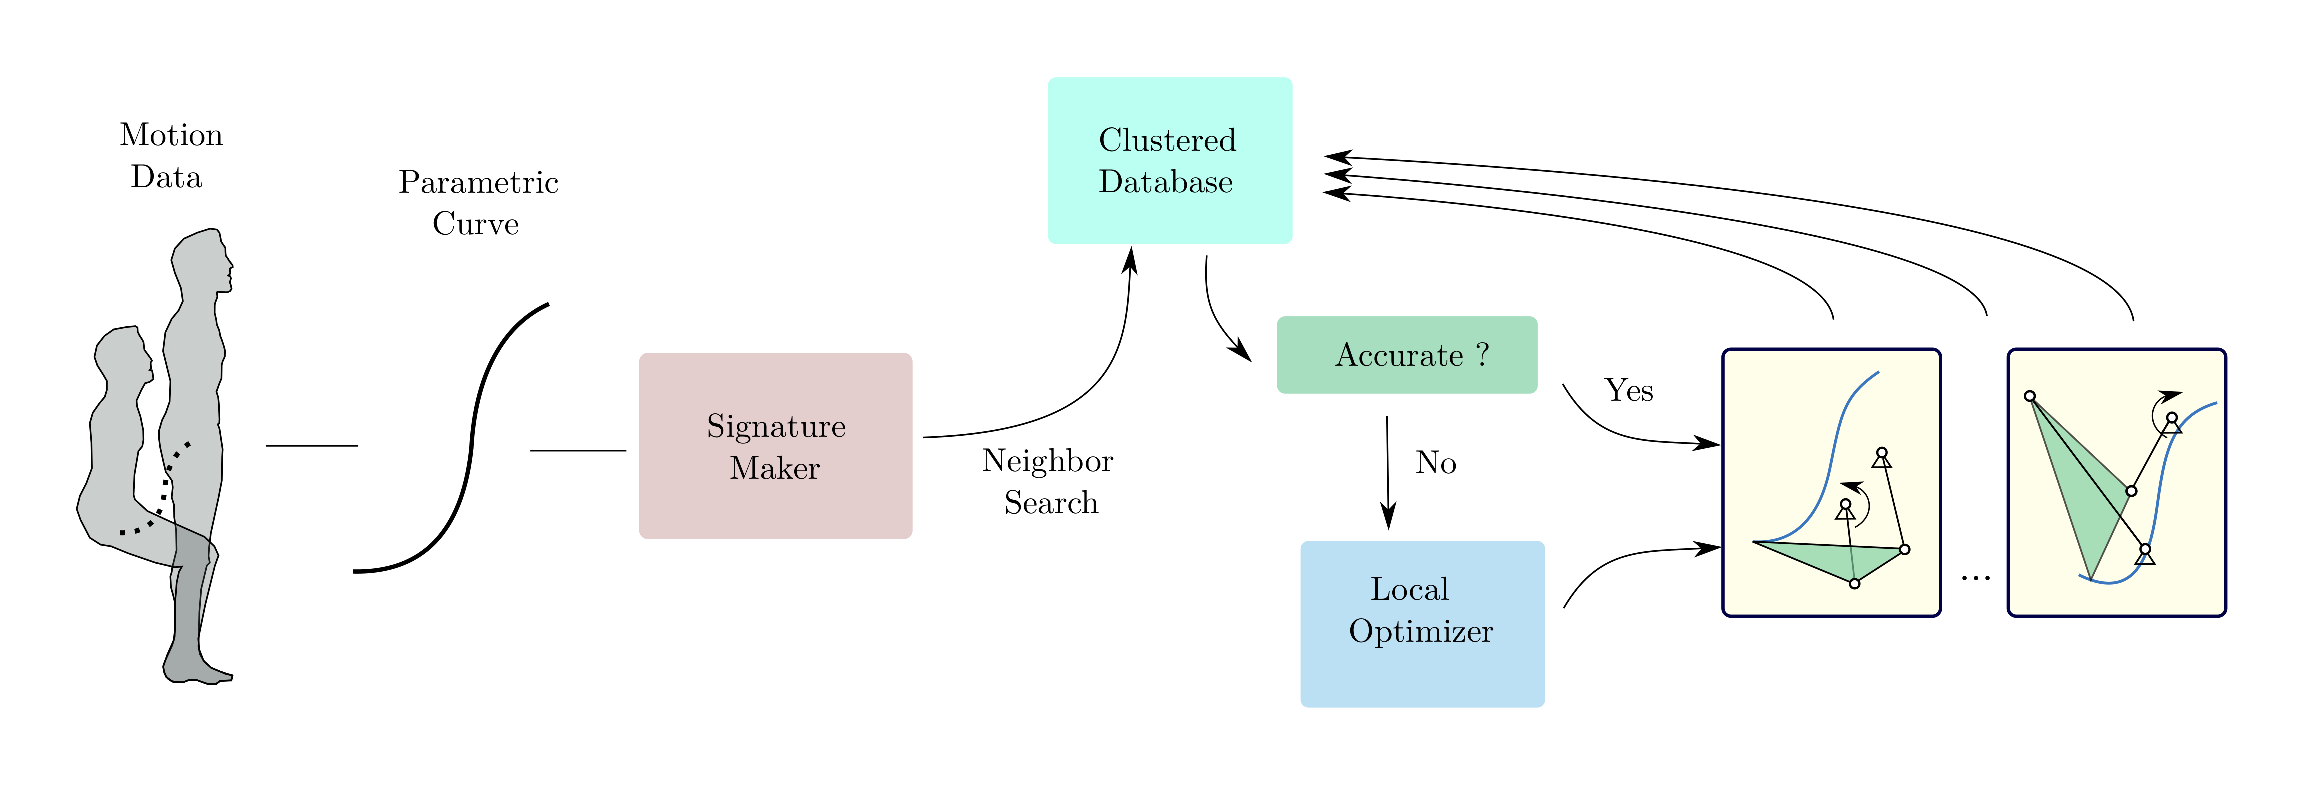
\includegraphics[width=\textwidth]{figure/overall_approach.eps}
  \caption{General Layout of the approach.}
\label{overallMethod}
\end{figure*}

Original contribution of this paper are in 1) a novel objective function for defect-free motion generation problem, 2) discovering a representation of coupler motion and path which is invariant under similarity transformations (henceforth termed as motion signature and path signature respectively), 3) novel algorithm for partial matching of motions , 4) optimal storage data by means of auto-encoder neural network and efficient neighbor search in the clustered database.
The objective function that drives the synthesis process, computes a distance measure of dissimilarity between the task motion and the coupler motion generated by current linkage parameters.
This distance measure of dissimilarity inherently requires continuity of motion; ensuring the output mechanism is defect free throughout the task.


Path synthesis methods based on Fourier analysis do take the continuity information of the coupler path into account, however majority of them are only defined on closed loop curves.
Ullah and Kota\cite{ullah1997} have presented an invariant approach towards representation and synthesis of closed paths through shape optimization. They use combination of global and local search methods by optimizing Fourier Deviant function to compute the dimensions of planar fourbar linkage without any initial guesses.
Wu et al.\cite{wu2011} presented a synthesis method for path generation based on finite Fourier series for synthesis of open and closed paths.
In the case of motion generation, methods that take the branching defect into consideration, limit their search in the configuration space where Grashof condition holds true.
To our best knowledge, no other motion generation method truly takes the motion continuity into account.

Owing to the highly nonlinear nature of the problem, most optimization based methods require good initial condition to start.
Thus, an atlas or a design library is used to provide good initial conditions.
McGarva\cite{mcgarva1994} has taken the earliest approach towards creating a library for coupler trajectories based on harmonic analysis.
Wandling\cite{wandling2000} has presented an atlas based approach, where coupler paths and motions are stored in terms of Fourier Transforms.
Input motion is searched for neighbors based on euclidean distances of Fourier Transforms.
Yue et al.\cite{yue-pathgen2011} presented a similar approach of path generation using P-Type Fourier Descriptor applicable for open curves.
In their approach, a task curve is transformed into normalized Fourier coefficients and queried for nearest neighbor search.
The best match is returned as solution to input. Chu et al.\cite{chu2010} have showcased an atlas based method of synthesizing spatial fourbar linkage for function generation problem where orientation data is stored in terms of Fourier harmonics.

The above methods generate data based on uniform sampling in the linkage parameter space.
Given the highly nonlinear mapping between linkage parameters and coupler trajectory, this way of sampling leads into non-uniform sampling of trajectory space causing under-representation of possible motions.
We try to address this issue by employing log normal distribution in the linkage parameter space to generate data and perform compact clustering of the data using machine learning techniques.
A Hierarchy is created in the database by means of clustering, where the top level comprises of few data points called cluster centers which are representative of the cluster points in the lower levels.
Also the methods\cite{wandling2000},\cite{yue-pathgen2011} have built the library with all possible coupler curves, where one curve is broken down into many segments for creating data for partial curves.
In contrast to this, we need to store only one curve representing all the segments in it as our representation facilitates partial matching.
No other previous method facilitates this partial matching of open motion curve into another open or closed curve.
Thus reducing the data requirement even further.

When a user inputs a motion or a path, a query representing invariant signature \footnote{path or motion signature} of the input is raised for k nearest neighbors among cluster centers in the database.
The neighbor is defined as motion or path whose part has a similar signature to the input. These k neighbors if needed, are subjected to fine tuning by local optimization to obtain set of solutions.
Overall method depicted in Fig.~\ref{overallMethod} is codified in Algorithm ~\ref{alg_overall}.

Organization of the paper is as follows. Section~\ref{sec_sign} presents the computation of motion and path signatures.
Section~\ref{sec_distanceMetric} is comprised of evaluation criterion for two signatures based on the shape similarity, which leads to form the error function for optimization.
Section~\ref{sec_SA} discusses the nature of objective function via sensitivity analysis at a singularity.
Section~\ref{sec_db_ae} explains the database generation and clustering using auto-encoders for efficient sampling and query operations.
Finally, two case studies are presented~\ref{sec_example} to showcase efficacy of the method.
%%%%%%%%%%%%%%%%%%%%%%%%%%%%%%%%%%%%%%%%%%%%%%%%%%%%%%%%%%%%%%%%%%%%%%

\begin{algorithm}
    \SetKwInOut{Input}{Input}
    \SetKwInOut{Output}{Output}
    \Input{Task Motion $\{x_i,y_i,\theta_i\}_{i=1}^{N}$ or Path$\{x_i,y_i\}_{i=1}^{N}$ }
    \Output{Linkage Parameters \emph{\textbf{l}: $l_1$, $l_2$, ...}}
    signature = calculateSignature(Input); \\
    distances = [];\\
    \For{centerPoint \textbf{in} clusterCenters}
    {
      distances.push(getDistance(signature, centerPoint))
    }
    kNeighbors = getNeighbors(distances, k)
    \For{neighbor \textbf{in} kNeighbors}
    {
      \eIf{threshold $<$ neighbor.distance}
      {
        \textbf{return} $neighbor.LinkParameters$
      }
      {
        \textbf{return} Optimize$(neighbor.LinkParameters)$
      }
    }
    \caption{Planar Linkage Synthesis}
    \label{alg_overall}
\end{algorithm}

%%%%%%%%%%%%%%%%%%%%%%%%%%%%%%%%%%%%%%%%%%%%%%%%%%%%%%%%%%%%%%%%%%%%%%
\section{Signatures of Coupler Path and Motion}\label{sec_sign}
The main focus of the paper is a novel method for motion generation that takes a continuous task motion or path as the input and returns defect-free linkages producing similar motion or path.
The objective function evaluation requires the input motion to be transformed into a specific form, which we call the signature of input motion.
This signature representation is invariant to similarity operations, which are reflection, rotation, translation and scaling.
Signature for path and motion are termed as path signature and motion signature respectively.
For calculating path signature we use formulations developed by Cui et.al\cite{cui2009}.
For this task, our approach requires the input in terms of a parametric motion $(x:x(t), y:y(t), \theta:\theta(t))$.
This section explains the procedure of signature calculation given in Algorithm ~\ref{alg_signature}.

\begin{algorithm}
    \SetKwInOut{Input}{Input}
    \SetKwInOut{Output}{Output}
    \Input{Twice Differentiable Parametric Representation of Motion $(x:x(t), y:y(t), \theta:\theta(t))$}
    \Output{signature //discretized signal in form of an array}
    k(t) = ComputeCurvature(x, y) using Eq.~\ref{curvatureEq} \\
    K(t) = IntergrateCumulatively(k(t)) using Eq.~\ref{kInt} \\
    motionSignature = [] \\
    pathSignature = [] \\
    \For{$i = 0 \to max(K)$}
    {
      tmp = (value of t corresponding to which K has value i) \\
      $i = i + 0.1$ \\
      motionSignature.push(k(tmp)) \\
      pathSignature.push(k(tmp))
    }
    \Return{PathSignature, MotionSignature}
    \caption{Calculate Invariant Signatures}
    \label{alg_signature}
\end{algorithm}

Curvature $k(t)$ of the path of a parametric motion $(x:x(t), y:y(t), \theta:\theta(t))$ and its integral $K(t)$ is given by,
\begin{eqnarray}
  k(t) = \frac{\ddot{y}(t)\dot{x}(t) - \ddot{x}(t)\dot{y}(t)}{{(\dot{x}^2(t) + \dot{y}^2(t))}^{(\frac 32)}}, \label{curvatureEq}\\
  K(t) = \int^{t}_0 |k(t)|dt \label{kInt},
\end{eqnarray}
where $\dot{x}$, $\ddot{x}(t)$ are first and second order derivative w.r.t. parameter t.
For an example, parametric motion could be a B-spline motion as shown in fig~\ref{bsplineFitting}.
We compute the curvature of path along the direction of t, using Eq.~\ref{curvatureEq} and the cumulative integral by Eq.~\ref{kInt}.
For implementation purposes, we use scipy\cite{scipy} module for computations of B-splines and their derivatives.
Figure~\ref{curvatureK} shows computed curvatures and its unsigned integral of coupler path shown in Fig.~\ref{bsplineFitting}.
It can be seen that curvature is very low at start, increases as the curve bends along the path and drops once again as the path straightens out.
It is obvious that curvature plot will reverse if the direction of parameterization reverses.

\begin{figure}
\centering
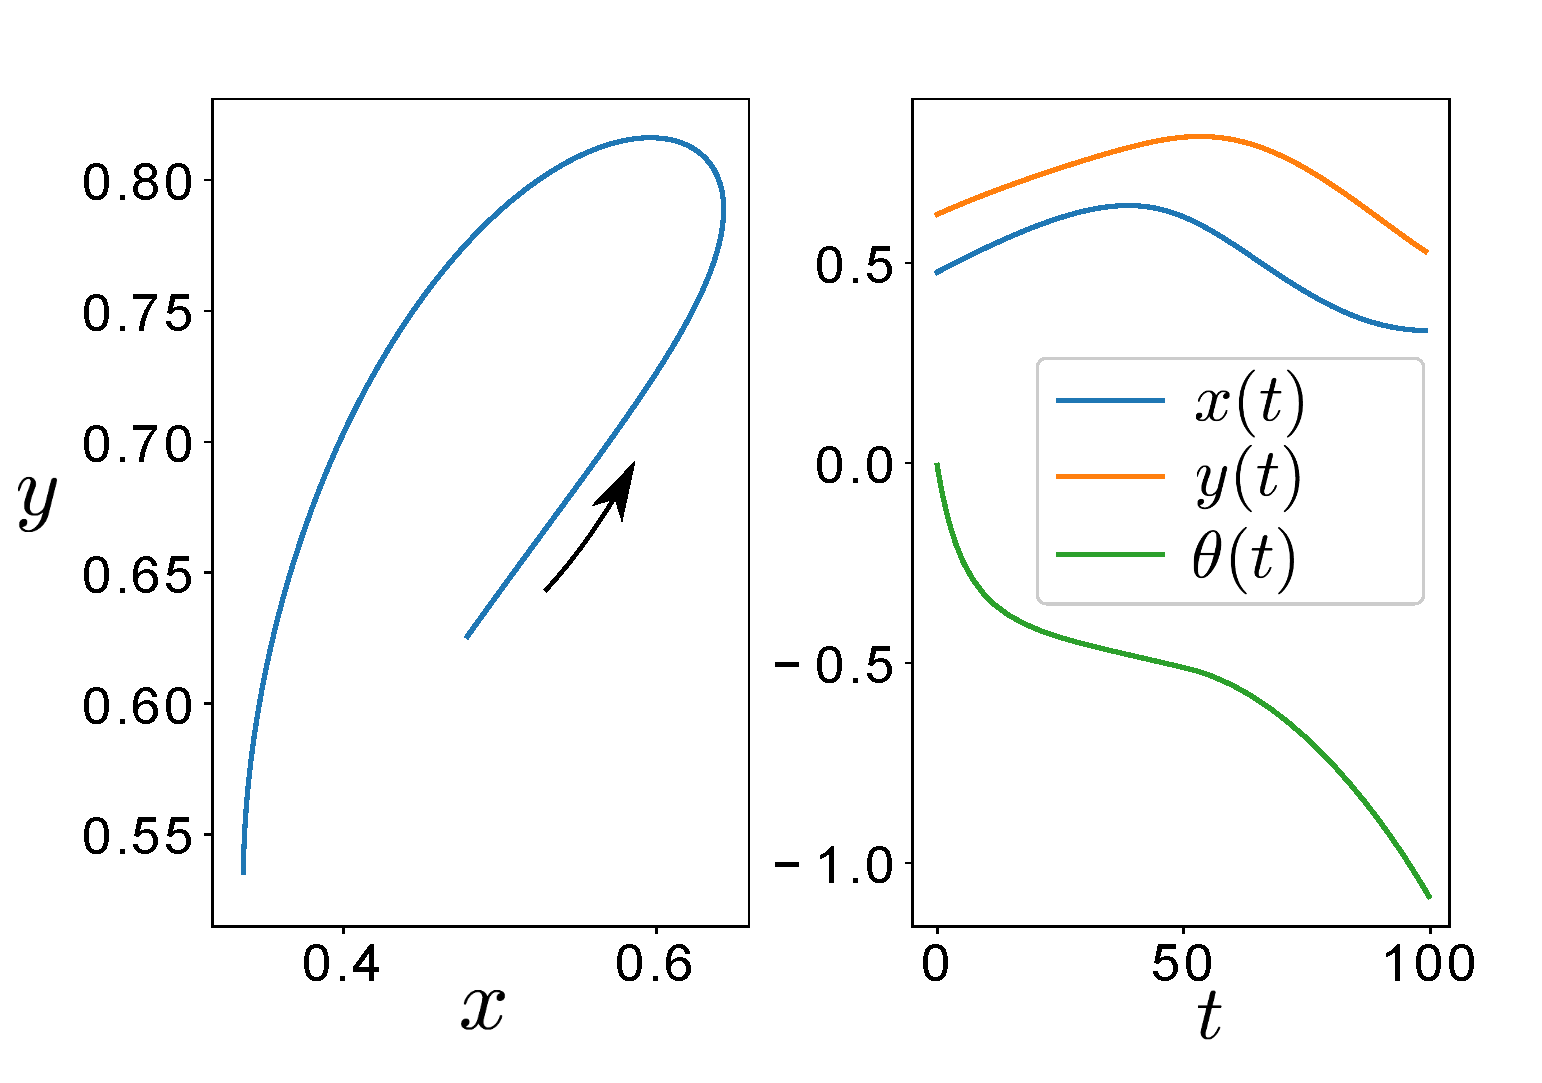
\includegraphics[width=240pt]{figure/fig_bspline.eps}
  \caption{a) The path of the input motion along with direction of parameterization. b) Motion components $x(t), y(t), \theta(t)$ are plotted against parameter t.}
\label{bsplineFitting}
\end{figure}

\begin{figure}
\centering
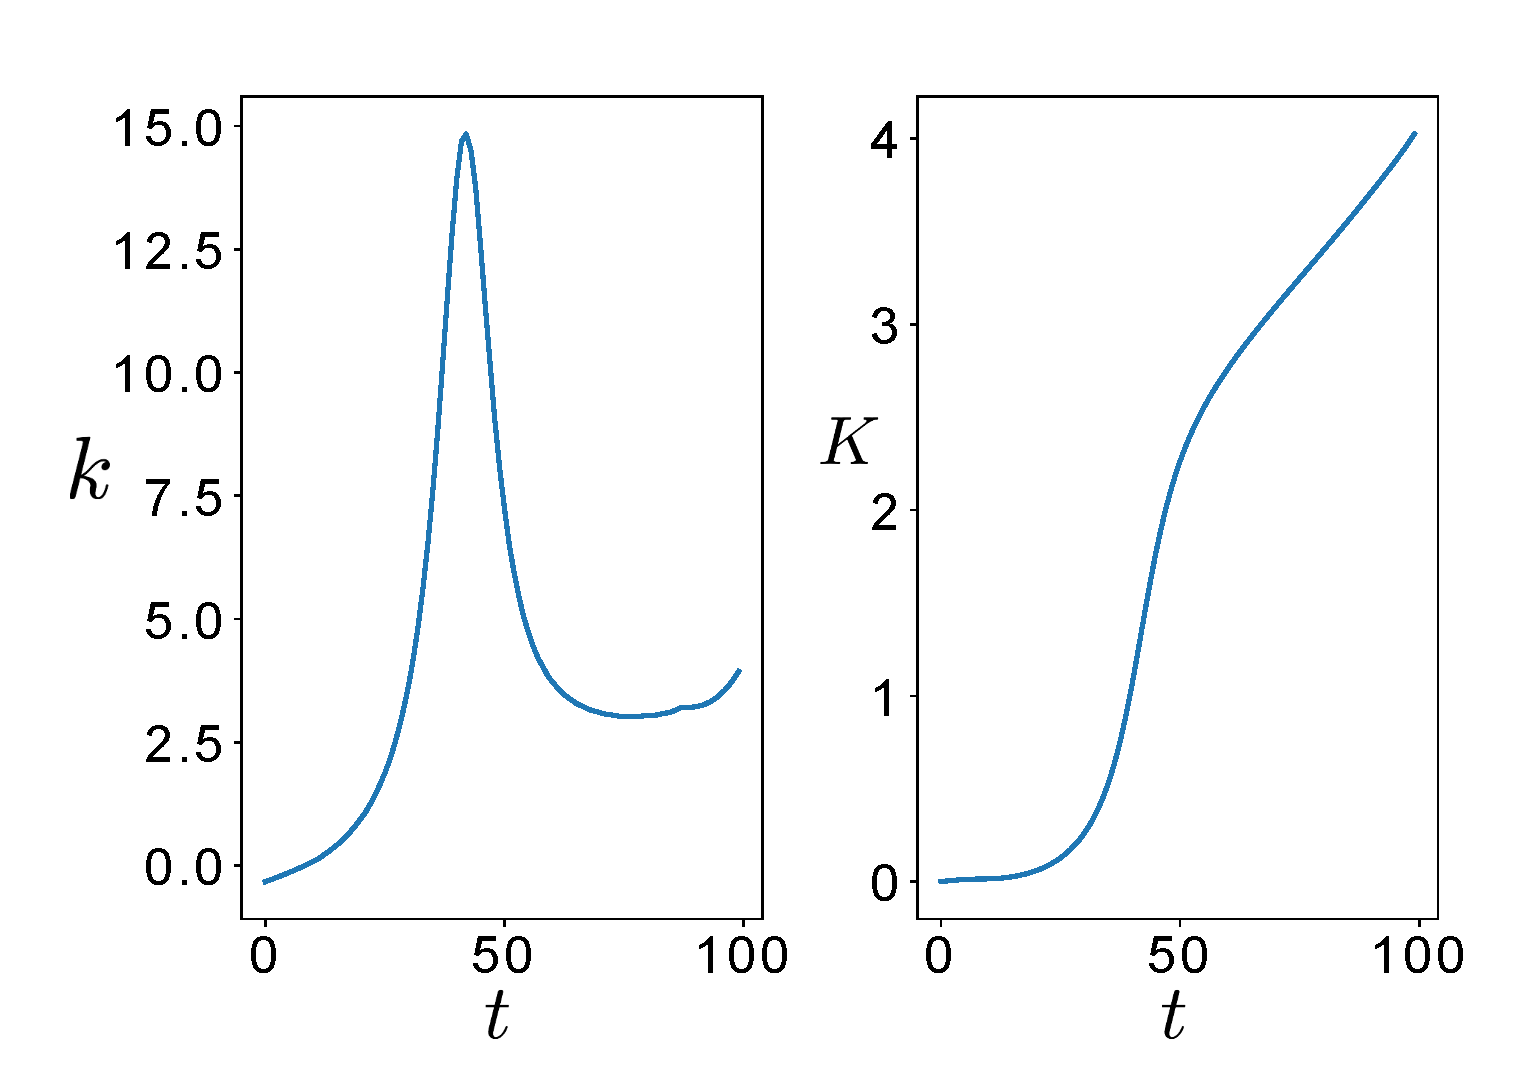
\includegraphics[width=240pt]{figure/fig_curvatureK.eps}
  \caption{Curvature and its unsigned integral for the path shown in Fig.~\ref{bsplineFitting}}
\label{curvatureK}
\end{figure}

Now we re-sample the curvature at equal intervals of $K(t)$, which is equivalent to plotting $k$ vs $K$ in Fig~\ref{signature}(a).
This is done by finding the parameter values of t where $K$ changes in the steps of some step size. For practical purposes we find array of parameter t such that $K$ increments by 0.1.
For each value of t in such array, we compute $k(t)$ and $\theta(t)$ and store it as the path and motion signatures respectively.

These signatures are invariant under similarity transformations; for proof see\cite{cui2009}.
The general intuition is as follows:
we know that curvature changes inversely to the scale of the curve, so when it is integrated along the scaled curve, the scale factor cancels itself out.
Reflection operation on the motion or the path, produces flipped path signature, but motion signature remains invariant.

Figure~\ref{signature} shows path and motion signature obtained for the motion depicted in Fig.~\ref{bsplineFitting}
It is important to note that signature depends on the direction along which we compute the curvature $k(t)$ as well as re-sample $\theta(t)$.

\begin{figure}
\centering
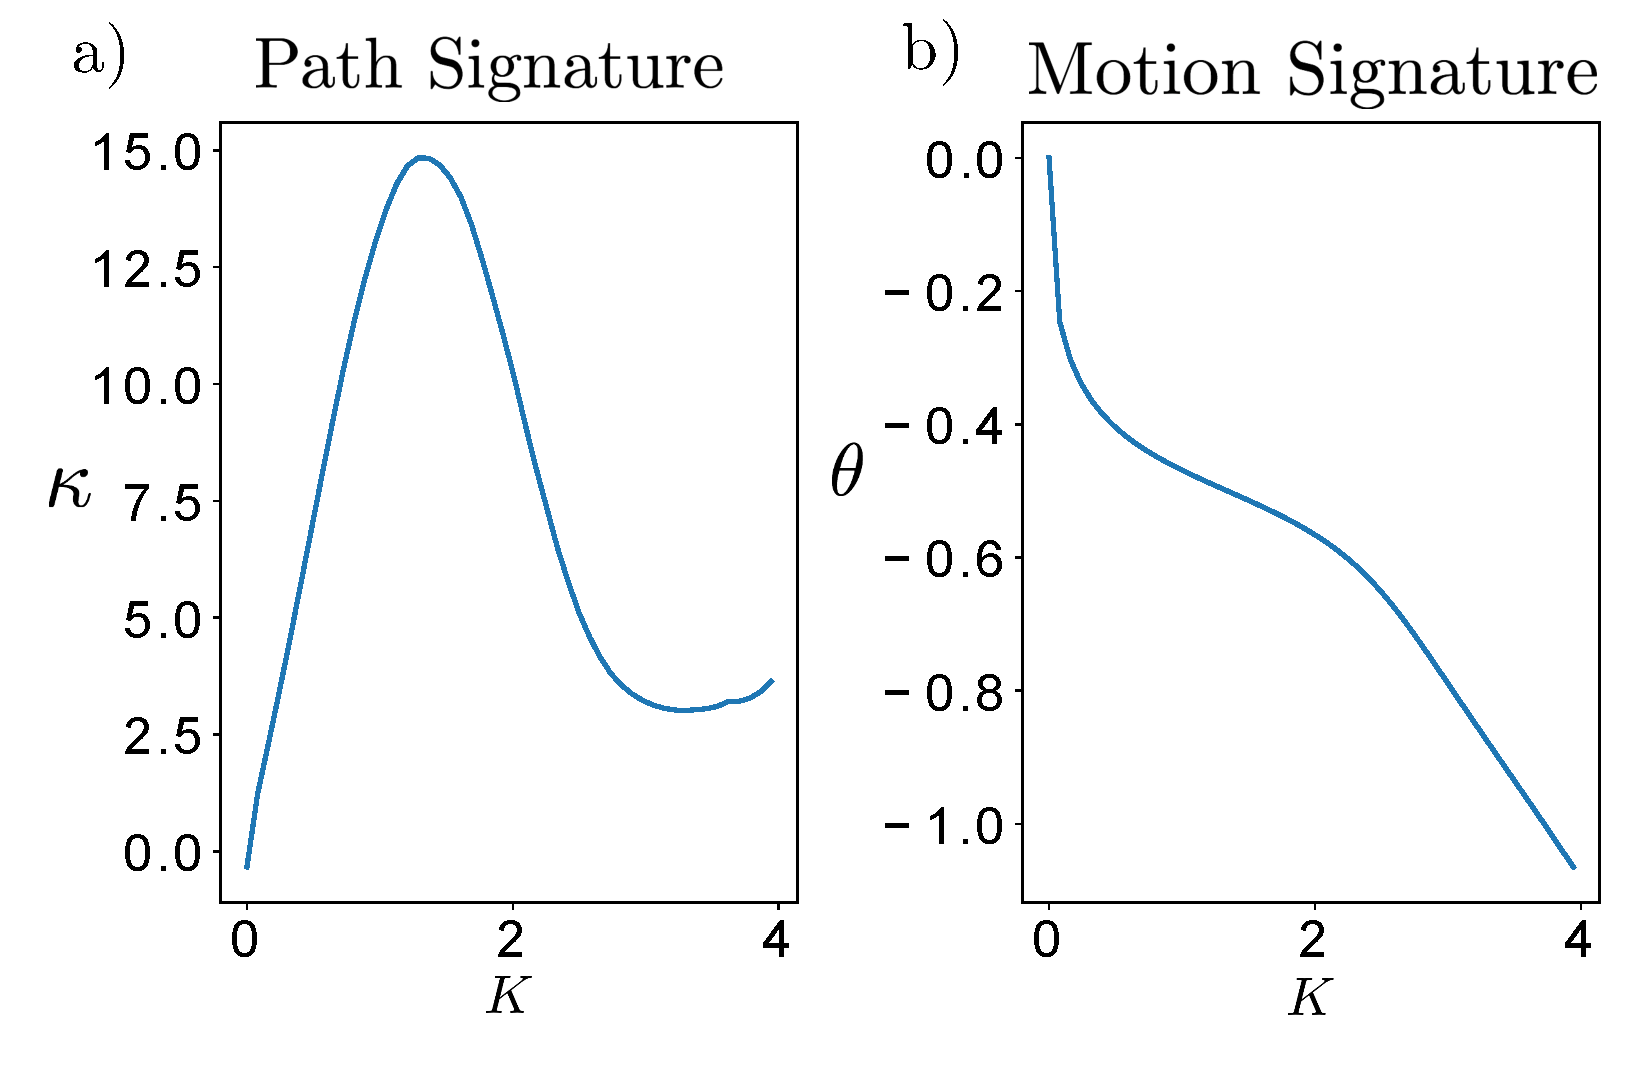
\includegraphics[width=240pt]{figure/fig_signatures.eps}
  \caption{Path and motion signatures of the motion shown in Fig.~\ref{bsplineFitting}}
\label{signature}
\end{figure}


\section{Signature Matching and Error Function}\label{sec_distanceMetric}
The signatures obtained in the previous steps contain important information about shape of the trajectory.
In this section we formulate functions that evaluate the similarity (or distance) between two trajectories based on their signatures.
These distance functions can be used as error metric which can be minimize using optimization methods.

\subsection{Partial Matching of Path Signatures}\label{sec_ncc}
When a path query is raised, it can be very useful to know whether this path already exists as a part in some other path present in the database.
This subsection presents a method for determining this partial similarity.

Lets consider two coupler paths; namely part and whole as shown in~\ref{wholePart}.
Let $p$ be path signature of the part path which acts as template, while $W$ is path signature of the whole path that can completely embed the template as shown in Fig.~\ref{pathSignature}. The orientation information shown in Fig.~\ref{wholePart}, is ignored for path matching. It will be used later for matching of motion signature.
The way this partial matching works is as follows:

\begin{enumerate}
  \item $p$ and $W$ are expressed in terms of arrays and $W$ must contain more points than $p$.
  \item The template $p$ is slid with offset index $j$ along $W$.
  \item For each offset $j$, we compute normalized cross-correlation function given by,
\end{enumerate}
\vspace{-0.6cm}
\begin{equation}\label{nccEq}
  Cn(j, p, W) = |\sum_{i}^{p_{span}} \frac{(W(i+j) - \bar{W}(j\to j + p_{span}))(p(i) - \bar{p})}{\sqrt{\sum_{i}^{p_{span}}{(W(i+j) - \bar{W}_{p_{span}})}^2\sum_{i}^{p_{span}}{(p(i) - \bar{p})}^2}} |,
\end{equation}
where $Cn(j, p, W)$ is the normalized cross-correlation value when template $p$ is matched against $W$ at $j^{th}$ index, $p_{span}$ is the length of the array $p$ and $\bar{W}(j\to j + p_{span})$ is the mean for the values of array $W$ between index range of ($j, j+p_{span}$)

Here $p$ acts as template that tries to find best match against $W$ while sliding over it along j.
Domain of $Cn(j, p, W)$ is [0, 1], where 1 represents the complete embedment.

Maximum score of the matching ($Cn_{max}(p, W)$) represents similarity of the template in $W$, and offset index $j$ at which maximum occurs is the start point for matching.
As the signature reverses with reversal of the direction of sampling, we compute the correlation first in one direction and again after reversing $p$ and select the best matching score, offset index and the matching direction of sampling.
Figure~\ref{ncc} depicts normalized cross correlation function over the sliding domain $j$ for part and whole curves.

\begin{figure}
\centering
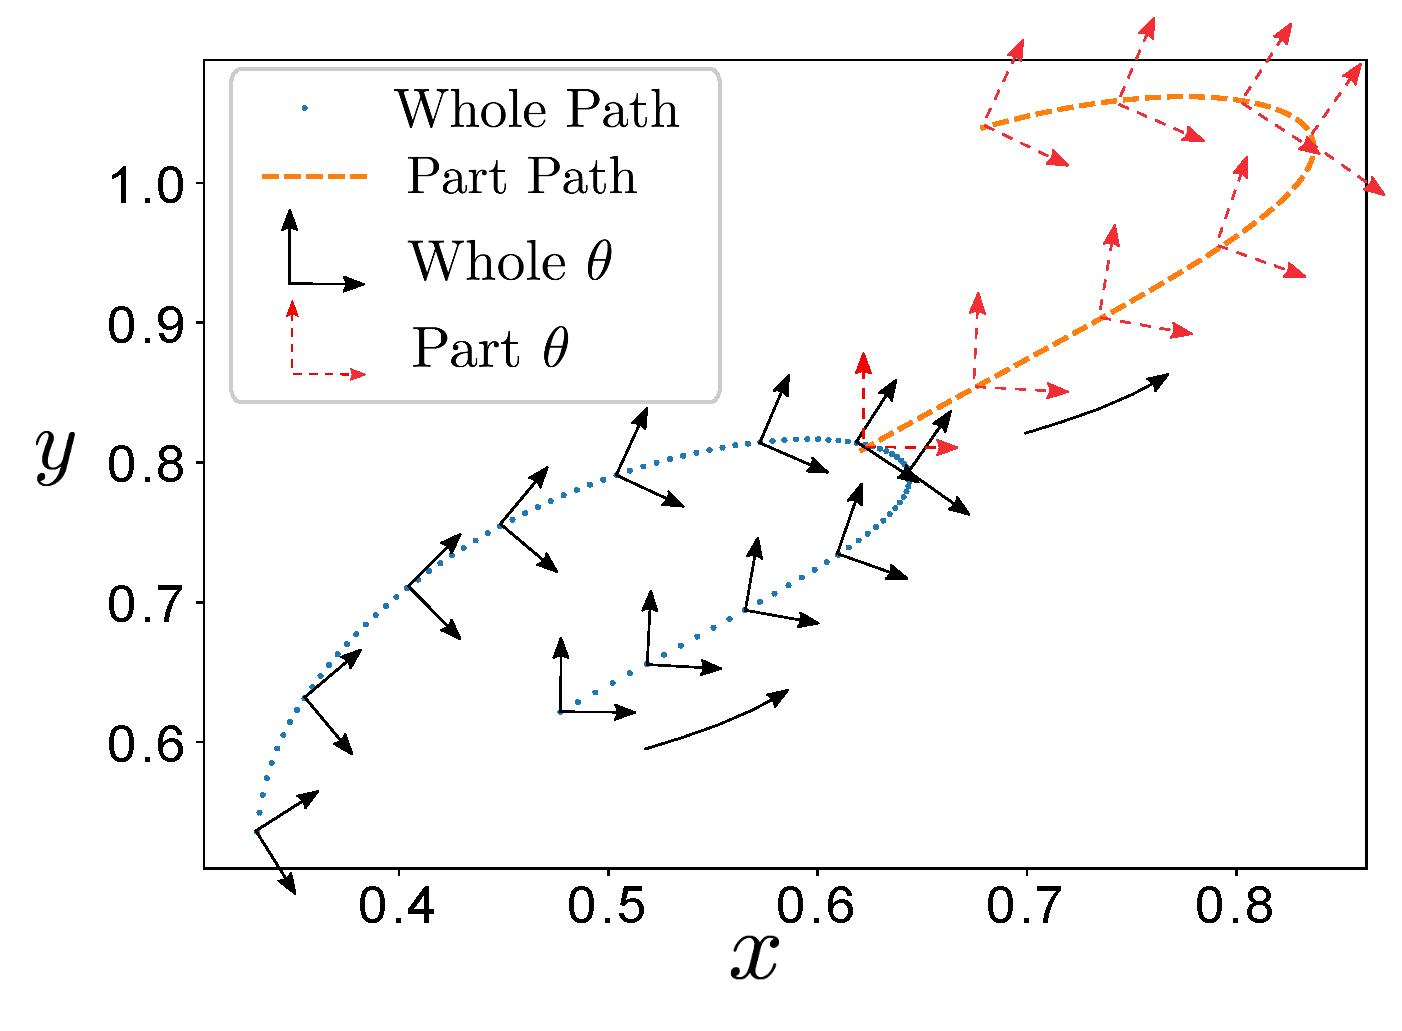
\includegraphics[width=240pt]{figure/fig_whole_part.eps}
  \caption{Part path is formed by trimming whole path followed by translation and scaling.}
\label{wholePart}
\end{figure}

\begin{figure}
\centering
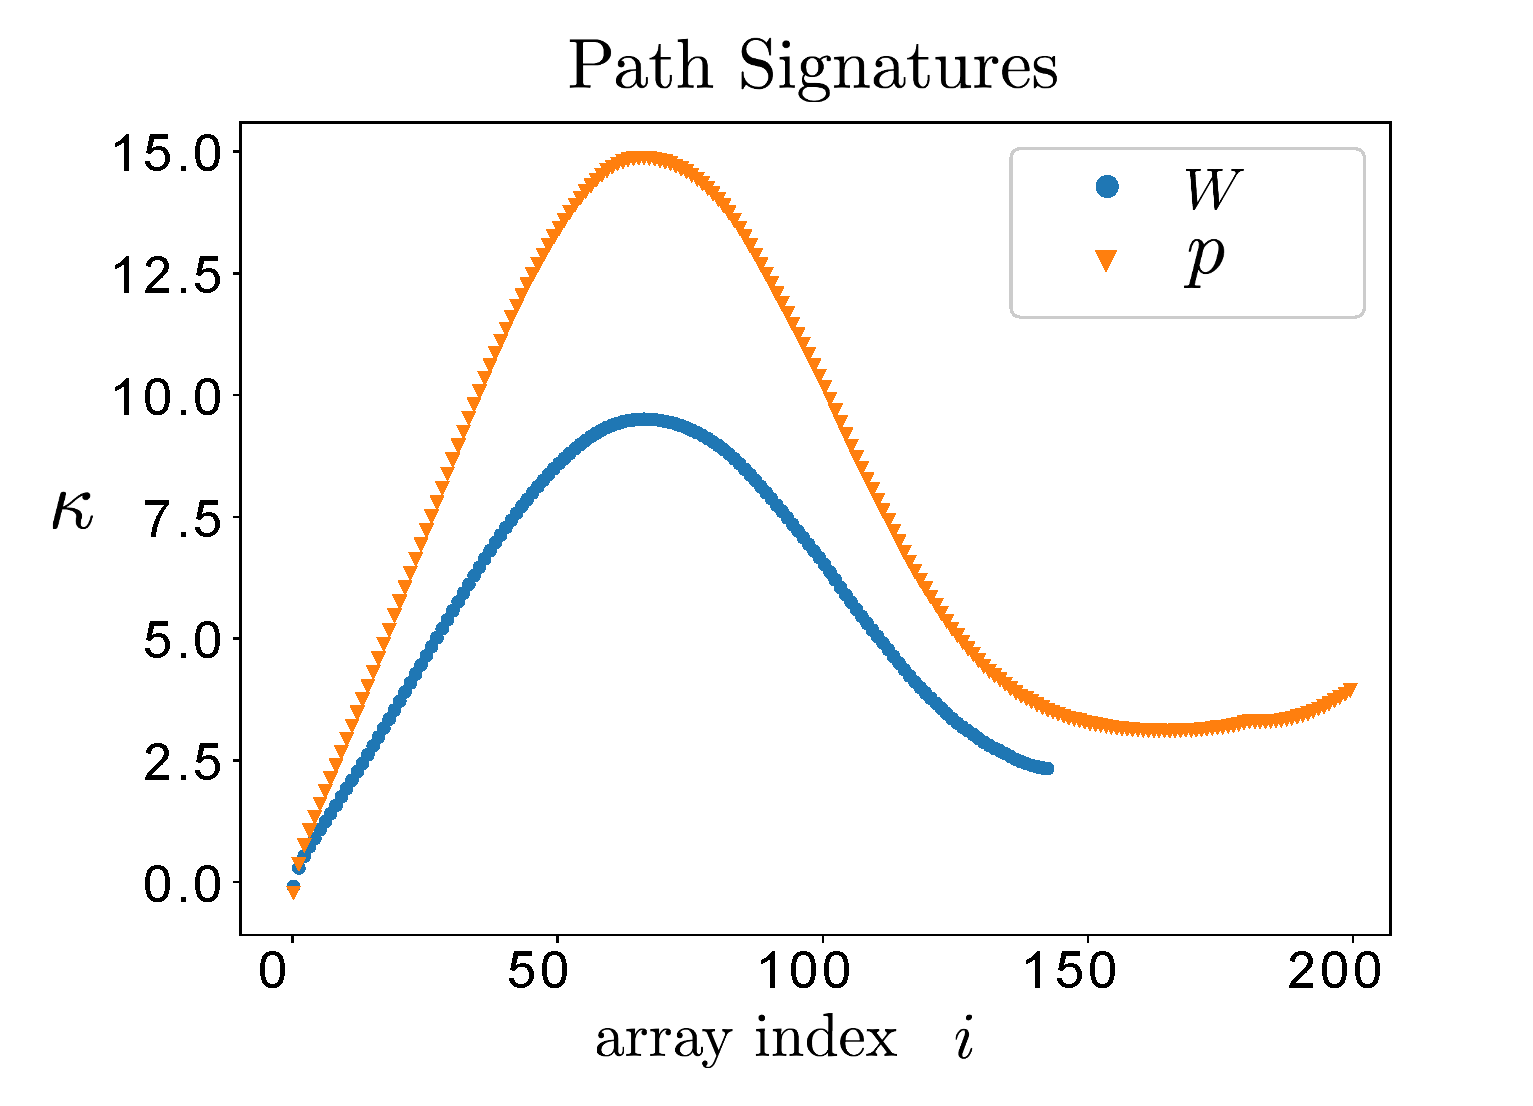
\includegraphics[width=240pt]{figure/fig_path_signatures.eps}
  \caption{Path Signatures of part $p$ and whole $W$ from Fig.~\ref{wholePart}.The domain of path signature is scale invariant but the range still has a scaling factor, which is taken care by normalized cross-correlation.}
\label{pathSignature}
\end{figure}

\begin{figure}
\centering
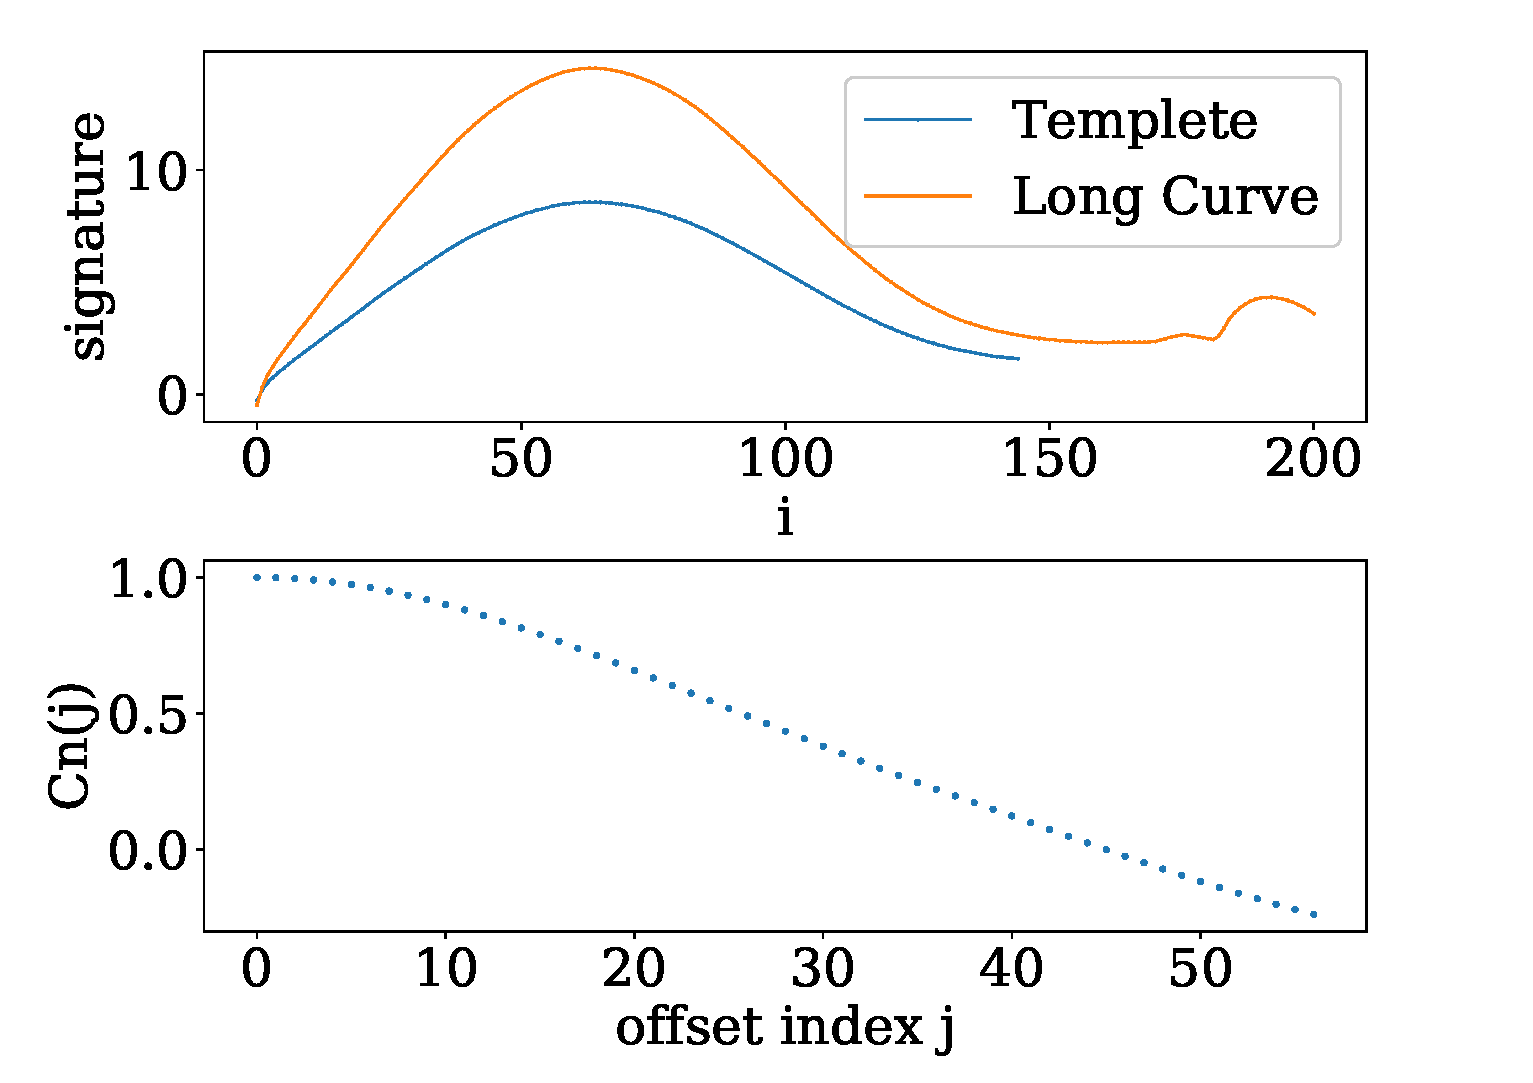
\includegraphics[width=240pt]{figure/fig_ncc.eps}
  \caption{Normalized cross correlation of the signatures computed along each direction is shown. It can be seen that exact match is found at $j=0$.}
\label{ncc}
\end{figure}

\subsection{Partial Matching of Motion Signatures}\label{sec_mcc}
This section presents how a template motion can be checked against other motion for potential matching.
Consider part and whole motions shown in Fig.~\ref{wholePart}.
Let $p$ and $W$ be the motion signatures of part and whole motions respectively.
All the steps are same as done for partial matching of path signature except the cross-correlation function which is given by,

\begin{equation}\label{mccEq}
  E(j, p, W) = \sum_{i}^{p_{span}} {((W(i+j) - \bar{W}(j\to j + p_{span})) - (p(i) - \bar{p}))}^2,
\end{equation}
where $E(j, p, W)$ is the dissimilarity value when template $p$ is matched to $W$ at $j^{th}$ index. Here $p$ tries to find best match against $W(i)$ while sliding over it.
Similar to path signature, motion signature is dependent on the sampling direction along the motion. Thus we compute the dissimilarity for both direction and the take whichever is the least i.e. $E_{min}(p, W)$.
Figure~\ref{mcc} depicts dissimilarity function over the sliding domain $j$.
In this case as shown in Fig.~\ref{mcc}, we find that the first point itself is a point where the perfect match is occurred, which is consistent with the fact that we slice the whole motion to obtain the part motion.

\begin{figure}
\centering
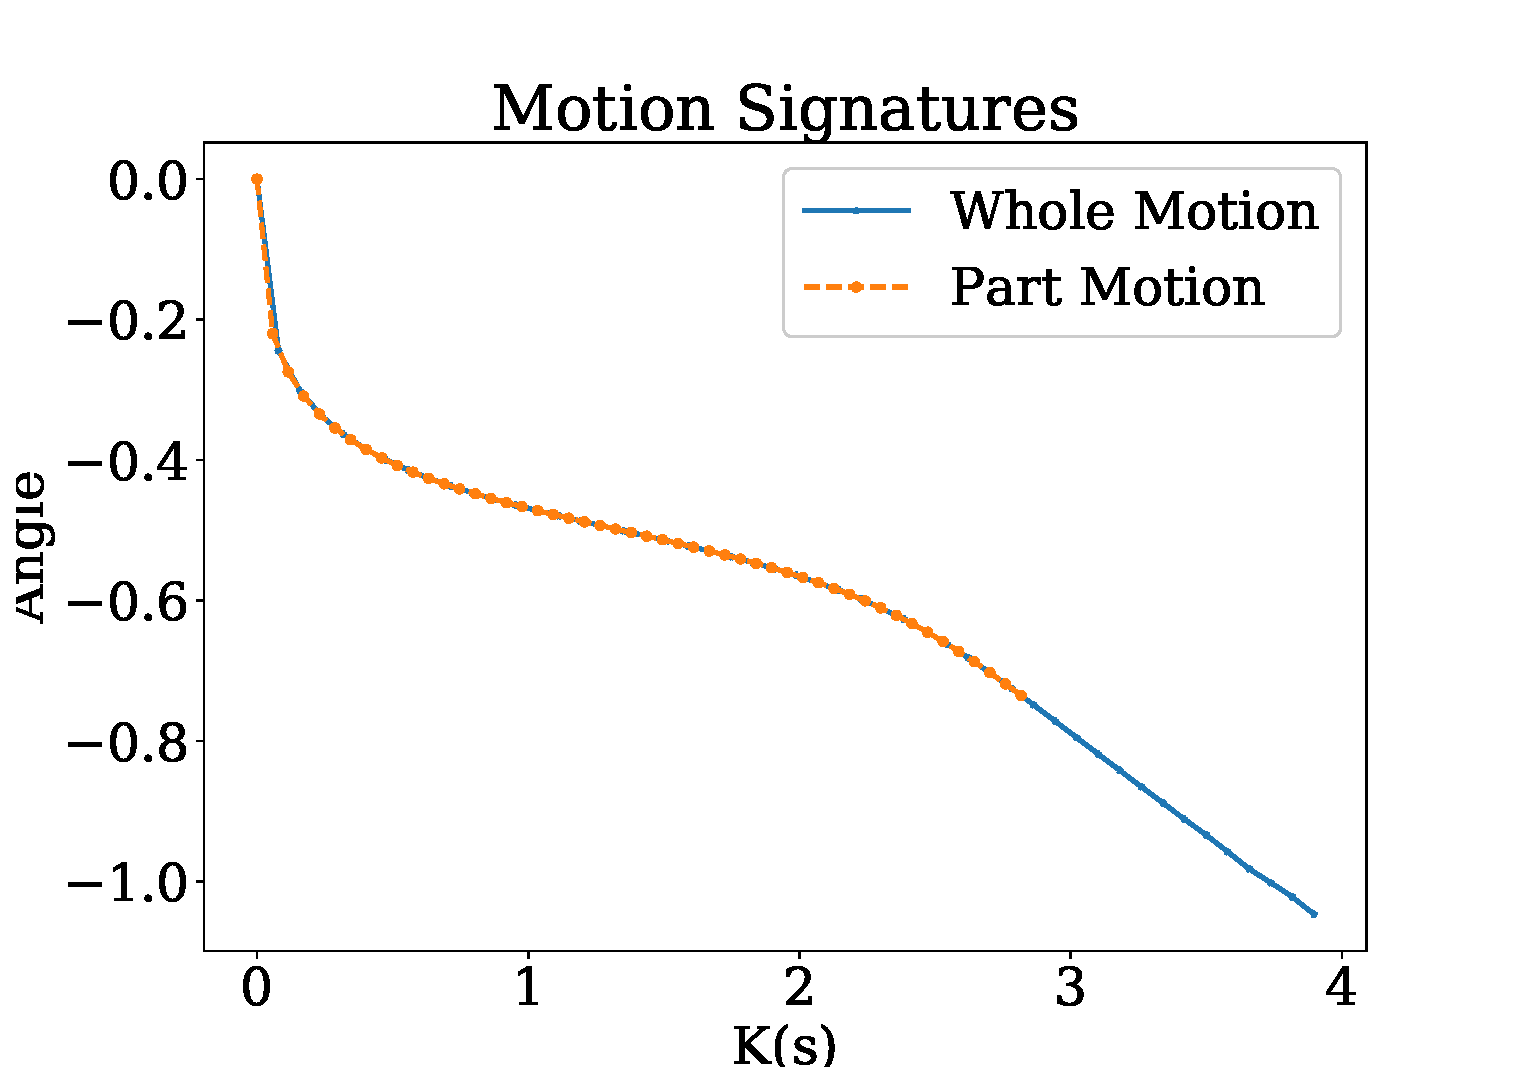
\includegraphics[width=240pt]{figure/fig_motion_signatures.eps}
  \caption{Motion Signatures of the trajectories shown in Fig.\ref{wholePart}. The domain as well as range of motion signature is invariant to similarity transformation.}
\label{motionSignature}
\end{figure}

\begin{figure}
\centering
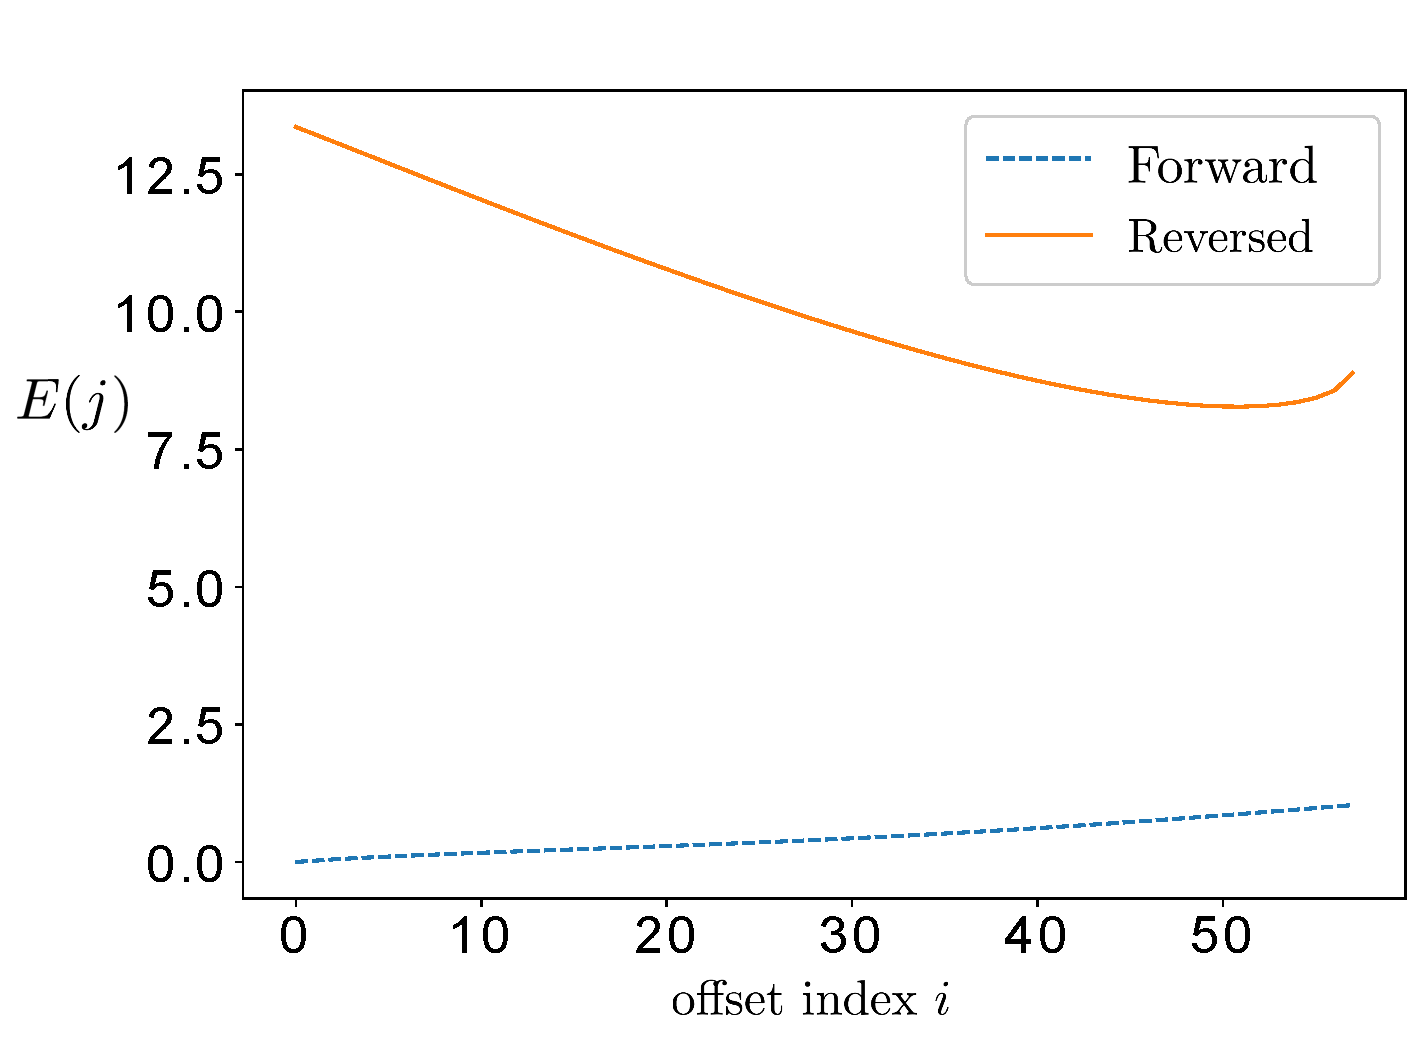
\includegraphics[width=240pt]{figure/fig_mcc.eps}
  \caption{Dissimilarity function of two motion signatures along both directions. It can be seen that exact match is found at $j=0$, where template is fully embedded inside the other motion.}
\label{mcc}
\end{figure}

\subsection{Objective Function for Synthesis}
The functions in Eq.~\req{nccEq} and ~\req{mccEq} presented in the sections \ref{sec_ncc}, \ref{sec_mcc} can be used as the error measure for path and motion synthesis of any planar linkage, where the objective is to find a linkage, that produces a motion whose part or whole corresponds to target motion (or path).
Thus we can formulate the path synthesis problem as,

\begin{equation}\label{objectiveFunPath}
  \argminA_{\textbf{\emph{l}}, W_i} (1 - Cn_{max}(p, W_i)
\end{equation}
where $\textbf{\emph{l}}$ is the vector of linkage parameters for particular planar linkage, p is signature the of task curve taken as template for Normalized Cross-Correlation and ${\{W_i\}}_{i=0}^{s}$ is the signature set of all $s$ coupler paths generated by the linkage corresponding to $\textbf{\emph{l}}$.
In case of four-bar, $\textbf{\emph{l}}: l_1, l_2, l_3, l_4, l_5$, with $l_i$ is link ratio of $i^{th}$ link shown in Fig~\ref{fourbar}.

Similarly, we can formulate motion synthesis problem as,
\begin{equation}\label{objectiveFunMotion}
  \argminA_{\textbf{\emph{l}}, W_i} (E_{min}(p, W_i))
\end{equation}
Here, E is the Dissimilarity function from Eq.~\req{mccEq} while p and ${\{W_i\}}_{i=0}^{s}$ are motion signatures instead of path signatures.

\begin{figure}
\centering
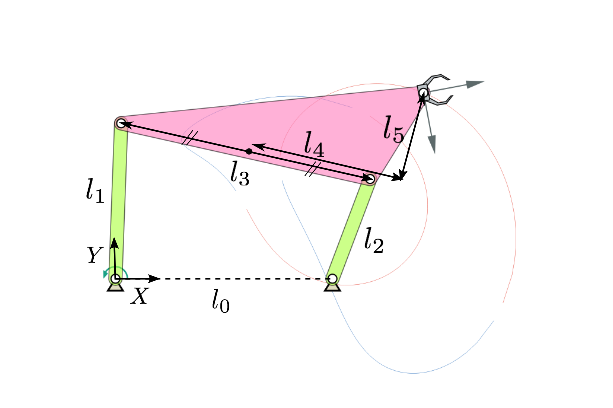
\includegraphics[width=240pt]{figure/fig_fourbar.eps}
  \caption{Parametric representation of four-bar linkage with all revolute joints. We set $l_0 = 1$ and one fixed joint at origin of the global frame along with making fixed length of the fourbar parallel to x axis.}
\label{fourbar}
\end{figure}

Objective function evaluation step consists of calculation of coupler motion or path and finding its dissimilarity score.
It is important to note that representation obtained in Section~\ref{sec_sign} reduces size of the linkage parameters in optimization.
This optimization problem can be solved using search methods which do not require gradient computation.
We can employ global optimization methods such as differential evolution at the start and local optimization methods link Powell's method towards the end for faster convergence\cite{ullah1997}.
%Section~\ref{examples} presents results for the optimization technique used.

Considering highly non-linear nature of the problem, finding a good initial guess proves to be game changing.
Thus we exploit machine learning techniques to create a database for finding many good initial guesses or the solution itself.

\section{Sensitivity Analysis of Signatures}\label{sec_SA}
Owing to the complex relationship between parameter space and generated motion, small change in linkage parameters can produce large and discontinuous structural change in the generated motions.
For example, small change in crank length ($l_1$) can open a previously close coupler path.
Most of the methods based on Fourier descriptors are if defined, can not capture the continuity at such singular locations, which adversely affect the optimization process.
In contrast to this behavior, the signatures derived in Sec.~\ref{sec_sign} have smooth transition at these singular locations due to shape similarity between a closed and just opened curve or motion.

To make our point, we perform sensitivity analysis as follows:
A four-bar with link ratios ($l_1:0.55$, $l_2:1$, $l_3:1.5$, $l_4:1$, $l_5:1$) is subjected to gradual change in parameters $l_1$ and $l_3$ by the amount (-0.2, 0.2) in steps of 0.01.
Error function between motions of new and initial fourbar are calculated using Eq.~\req{objectiveFunMotion} .
Figure~\ref{saCouplerCurves} shows coupler motion of some of the four-bars while Fig.~\ref{saMotionSignatures} depicts their motion signatures.
It can be seen from Fig.~\ref{saCouplerCurves} that there exists a discontinuity in topology of the coupler curves even though their shapes have a continuous shift.
Our method captures this continuity, which is shown by error function evaluations depicted in Fig.~\ref{saErrorFunction}, where it is visible that surface is well behaved in the singularity region.

\begin{figure}
\centering
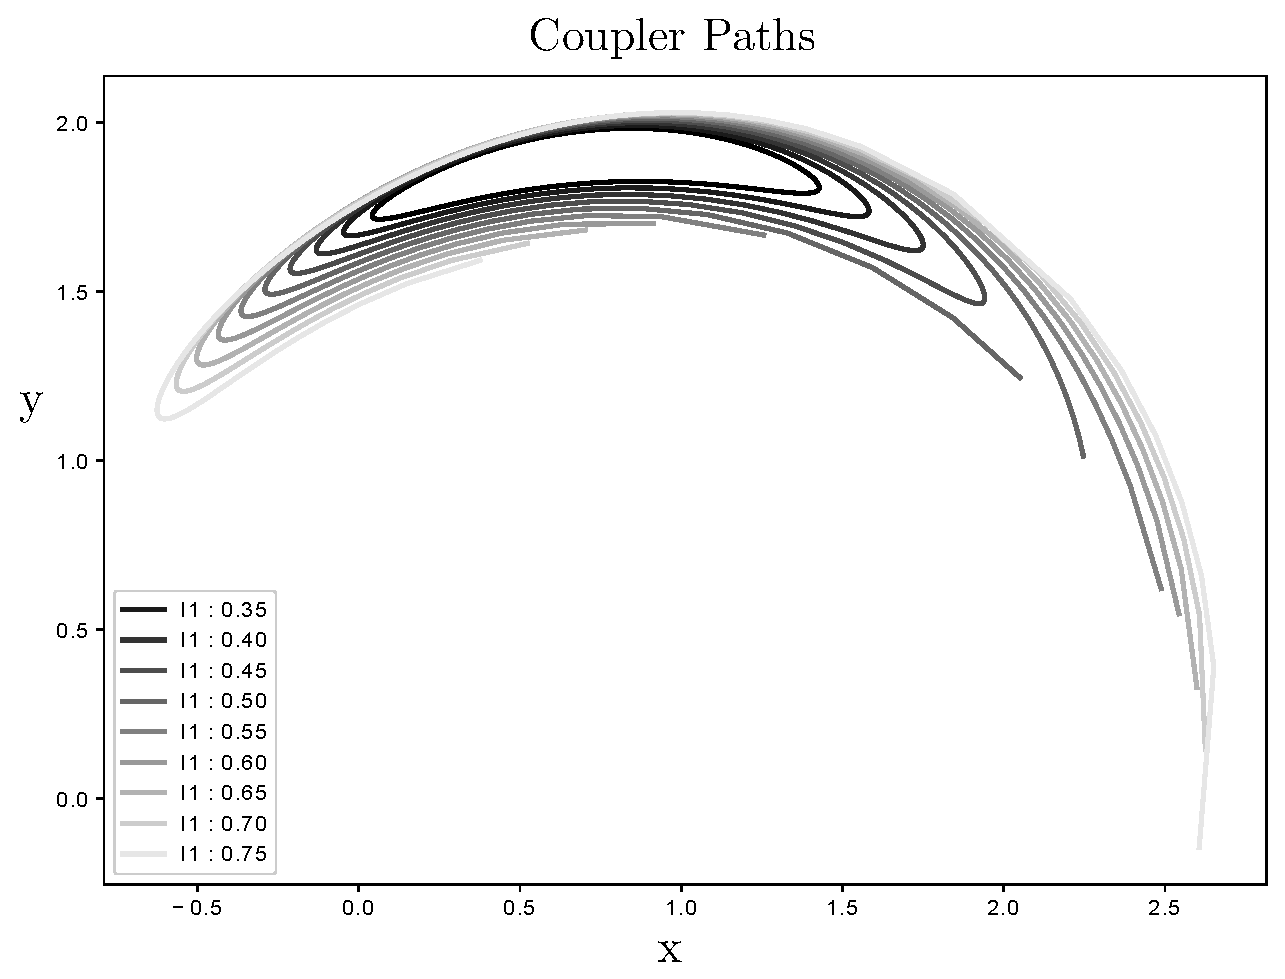
\includegraphics[width=240pt]{figure/fig_sa_coupler_curves.eps}
  \caption{Coupler Motions of the fourbar linkage with variation of parameters $l_1$ and $l_2$. It can be seen that motion topology changes from close-loop Grashof to open loop Triple-Rocker.}
\label{saCouplerCurves}
\end{figure}

\begin{figure}
\centering
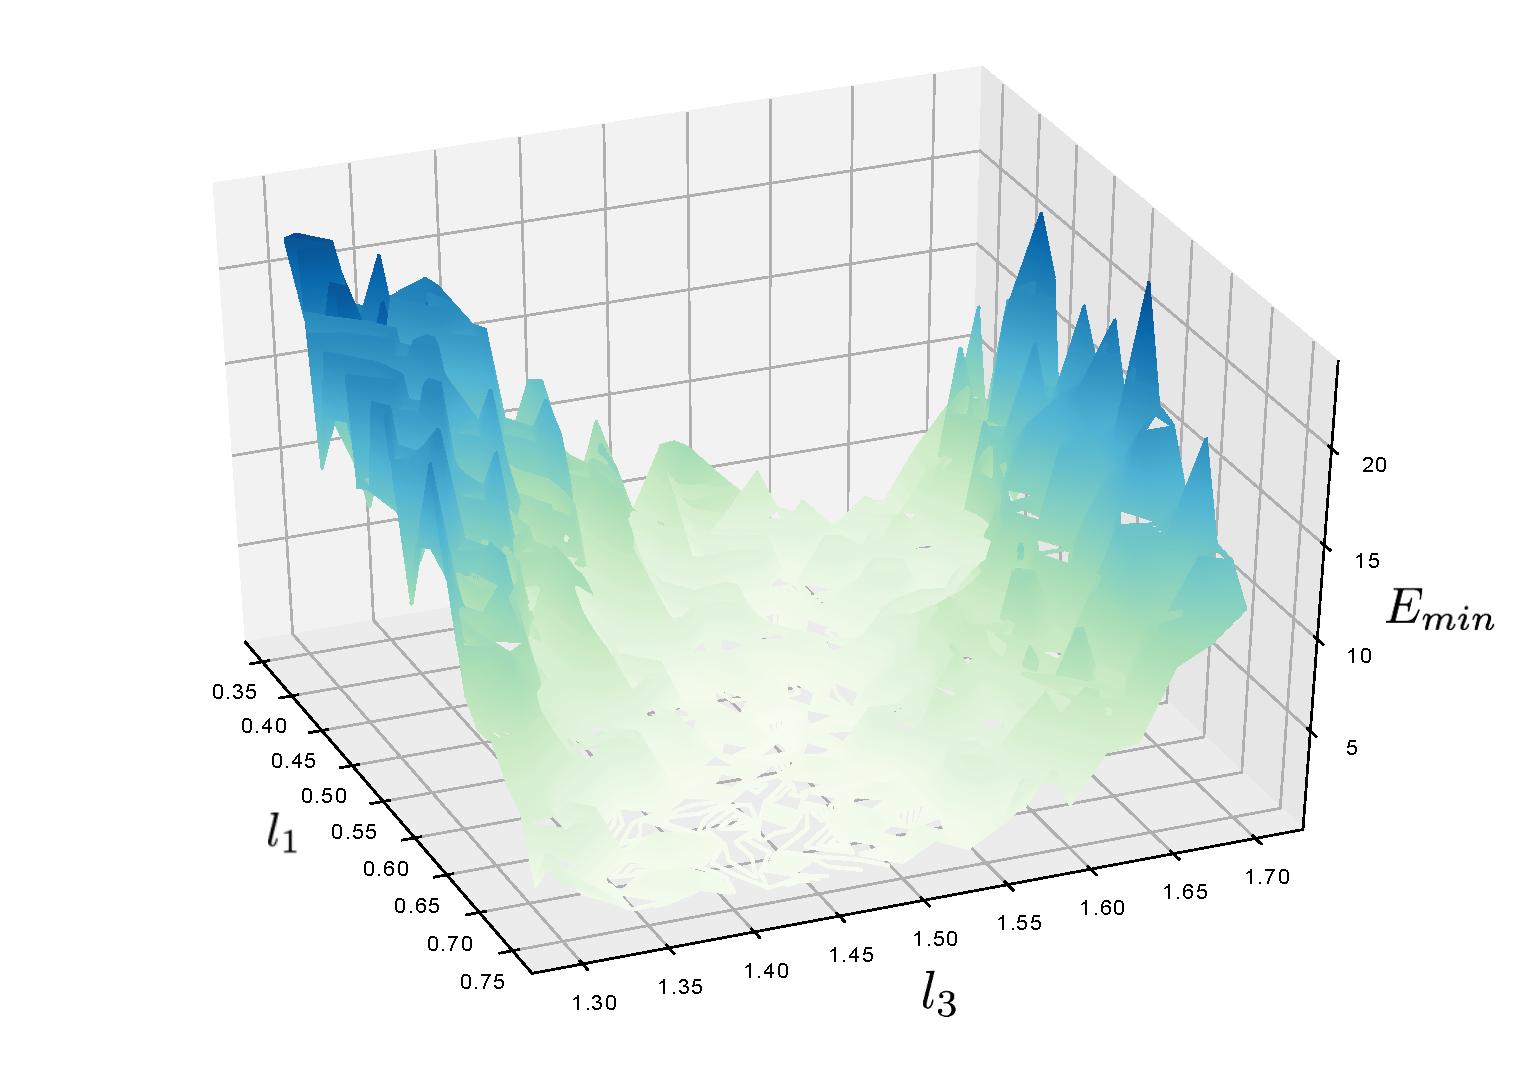
\includegraphics[width=240pt]{figure/fig_sa_distance_function.eps}
  \caption{Distance ($E_{min}$) from Eq.~\req{mccEq} as the parameters $l_1$ and $l_2$ are varied. Although open loop breaks at $l_1$:0.55, $l_3$:1.5, there are no spikes of error function in the region near singularity, as the shape is very similar between the two topologies.}
\label{saErrorFunction}
\end{figure}

\begin{figure}
\centering
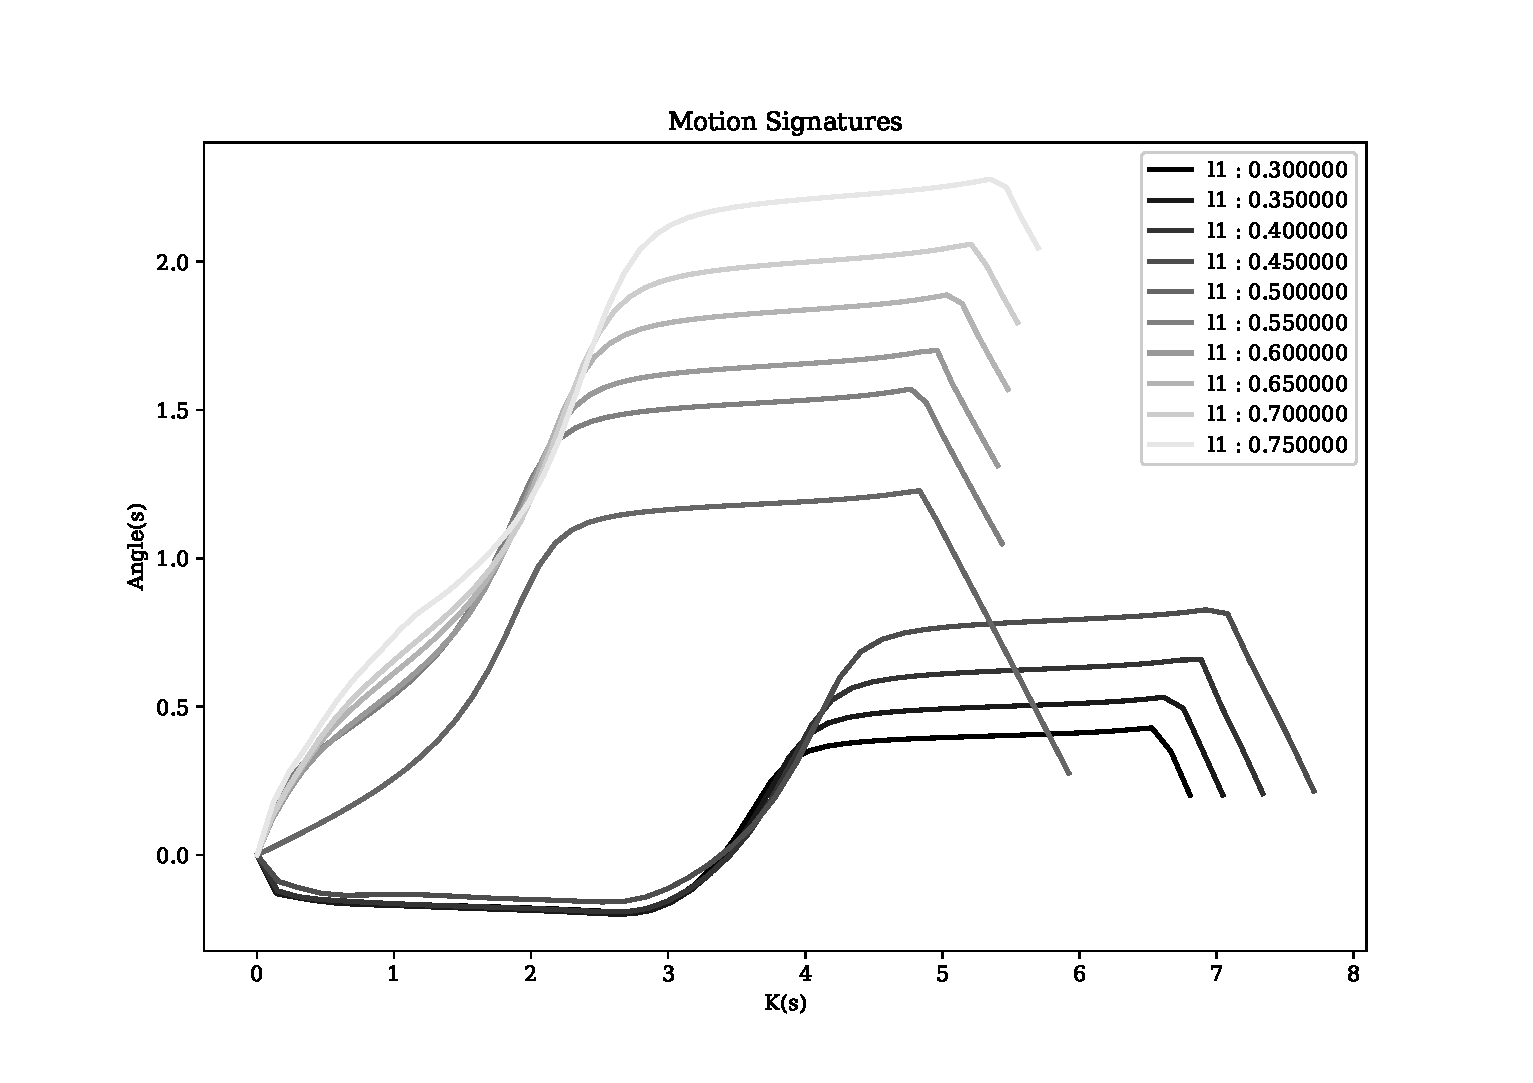
\includegraphics[width=240pt]{figure/fig_sa_motion_signatures.eps}
  \caption{Motion signatures obtained by steps given in~\ref{sec_sign}. Although topology difference is even more evident in this representation, it also signifies the similarity pattern between them.}
\label{saMotionSignatures}
\end{figure}

\section{Clustered Database of Planar Linkages}\label{sec_db_ae}
Having a invariant representation facilitating partial matching greatly reduces data required to sample all possible types shapes of coupler motion.
We have built a database of planar four-bar linkages with revolute joints as an example, but the approach is same for any planar motion generating machine.
We generate this database comprising of $40,000$ linkages, while taking following aspects into consideration.
\begin{enumerate}
  \item Sampling should maximize the uniformity of its distribution over the space of four-bar coupler motions.
  \item Data generation can be parallelized.
  \item Scalable with linkages with more number of links.
\end{enumerate}
Figure~\ref{fourbar} represents parametric representation of four-bar linkage with parameters ($l_1,l_2,l_3,l_4,l_5$).
As mapping between four-bar linkage parameter space and coupler motion space is highly non-linear, uniform distribution over linkage parameter space doesn't necessarily mean uniform sampling over motion space.
Thus the efficient approach would be to sample more in the regions where sensitivity is maximum.
Our observational intuition tells that whenever the link ratios of four-bar linkage are close to 1, the sensitivity of the shape of a coupler motion is higher than otherwise.
Thus we have chosen Log-Normal probalitiy distribution ($\mu = 0,\sigma = 0.6 $) for selecting the link ratios : $(l_1, l_2, l_3)$ as shown in Fig.~\ref{logNormal}, and Normal Distribution ($\mu = 0,\sigma = 2 $) for $(l_4, l_5)$.

\begin{figure}
\centering
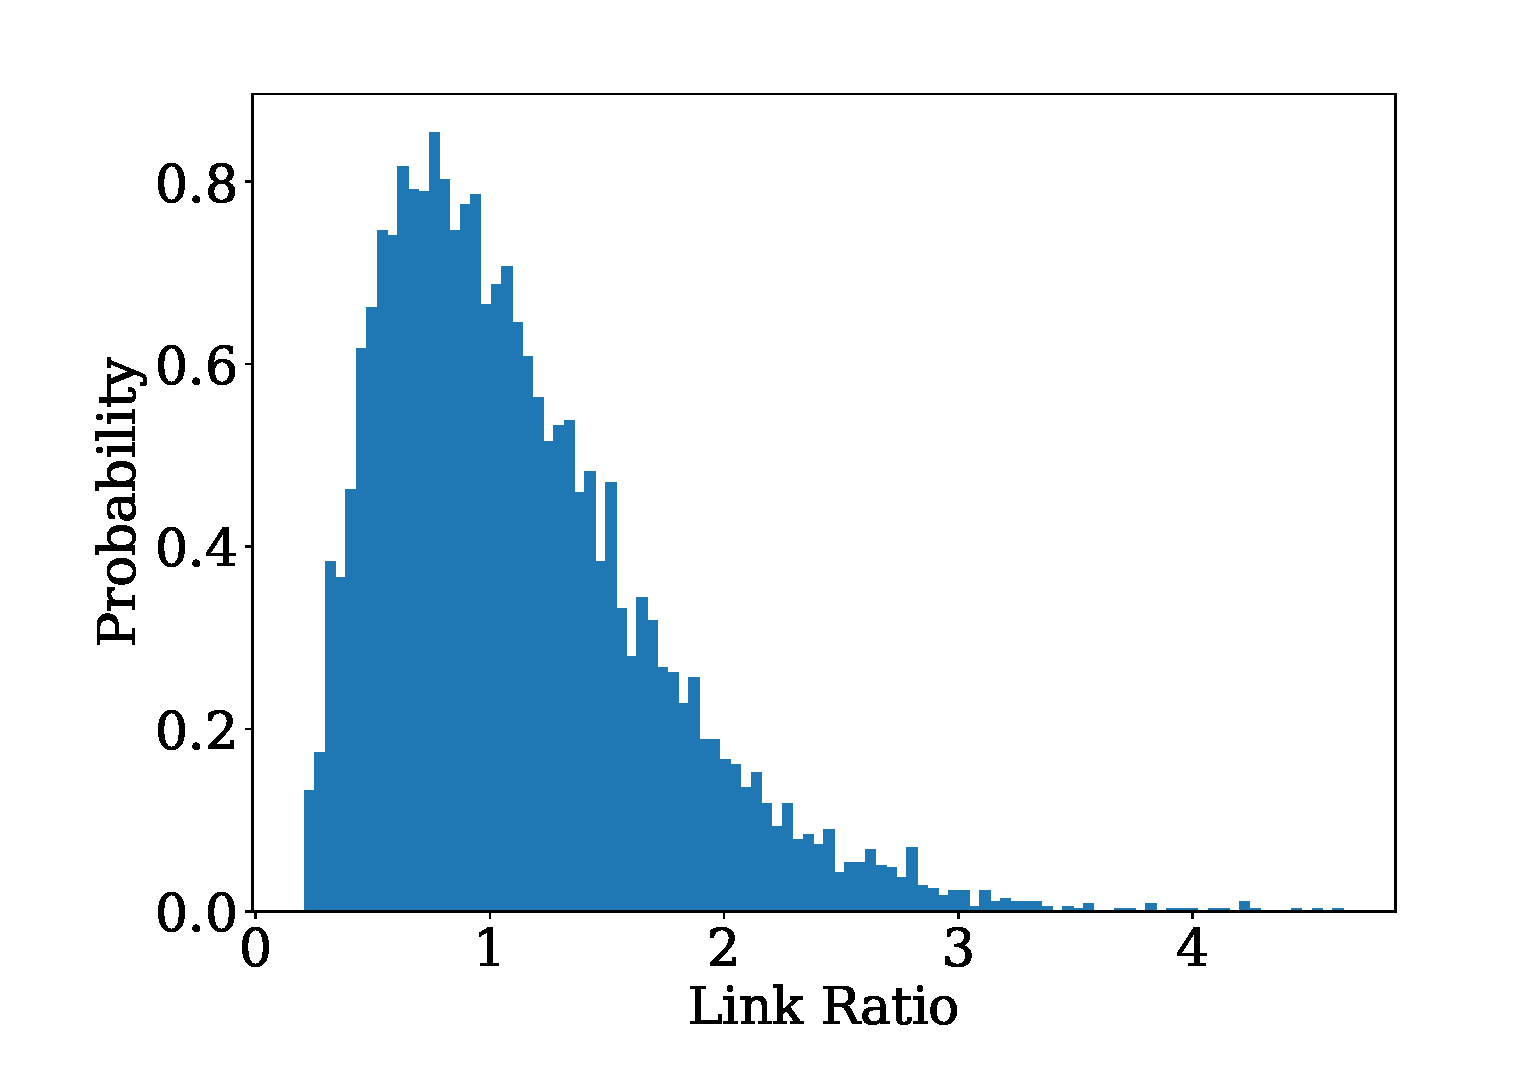
\includegraphics[width=240pt]{figure/fig_logNormal.eps}
  \caption{Probability Distribution function used in random sampling for parameters $l_1$, $l_2$ and $l_3$.}
\label{logNormal}
\end{figure}

\subsection{Dimensionality Reduction using Auto-Encoders}
Each data point in database consists of discrete signature of motion, which is kept to be of 100 float digits.
In order to have efficient query operations, we perform Hierarchical Clustering; a method that summarizes and creates a hierarchy in the database.
Clustering in higher dimensions suffers from \emph{Curse of Dimensionality}\cite{marimont1979}, thus we first perform dimensionality reduction using Auto-encoder Neural Networks.
Auto-encoder is a powerful mapping model, which learns to encode the input data in very compact representation and can reconstruct the input with minimal error; performing much better than Principal Component Analysis\cite{hinton2006}.
This Non-linear mapping by auto-encoder can greatly improve the representation of data for clustering (For details refer \cite{song2013}).
Figure~\ref{autoEncoder} shows a Neural Network architecture similar to the one we designed for the task.
Our architecture consists of 100 neurons in input and output layer, while five hidden layers have (80, 50, 10, 50, 80) neurons respectively.
Each neuron in the hidden layer is activated by Rectified Linear Unit (\emph{ReLU}) activation function.
In $i^{th}$ hidden layer, $d^{(i-1)}$ dimensional vector output of the previous layer $h_(i-1)$ is fed as input to produce $d^{(i)}$ dimensional output $h_i$.
Input-output relationship of a layer is given by,

\begin{eqnarray}\label{nnlayer}
  h_i = ReLU(W_{i}h_{i-1} + b_{i}), \\
  ReLU(x) = max(0, x),
\end{eqnarray}
where $W_i$ is weight matrix with dimensions $(d^{i}, d^{(i-1)})$ and $b_i$ is $d^{(i)}$ dimensional bias vector of $i^{th}$ layer, which are computed in the process of training.
Auto-encoders are trained to reconstruct the input, in this way each layer encodes the input, which is sufficient for the next layers to reconstruct the output.
Objective of the training is to find out set of weights and biases that minimizes the error loss given by,

\begin{equation}\label{nnloss}
  \argminA_{W, b} \sum_{i=0}^{N} || X_i - \tilde{X}_i ||^2,
\end{equation}
where $X_i$ is input, $\tilde{X}_i$ is reconstructed output and N is number of training examples.


Once a network is trained, Output of the bottle-neck layer $(h_{ib})$ represents the compressed feature space ($Z$).
As the bottleneck layer has 10 neurons and input is 100 dimensional vector, it is evident that information is compressed by a factor of 10, while achieving $95\%$ reconstruction accuracy as a result of training.
Standard clustering algorithms are performed on this latent\footnote{compressed output of bottleneck layer.} space for better clustering\cite{song2013}.
We use Agglomerative Clustering, a method of Hierarchical clustering, which is an approach to partitioning clustering for identifying groups in the dataset.
\emph{Ward}\cite{ward1963} criterion is used for clustering, which minimizes the variance of the clusters being merged.
The distance metric used is the euclidean distance in the latent space.
Although the more accurate distance metric is distance function discussed in sec.~\ref{sec_distanceMetric}, it is very expensive to calculate it for entire database.
Signatures with ${O}(m)$ points, take ${O}(m\log{}m)$ time for each comparisons and there are ${O}(N^2)$ number of comparisons to be made for database of $N$ points.
When user raises one such query, we first find k nearest neighbors among $1500$ cluster centers, then descend into their clusters if needed.
Motion with highest similarity score is returned along with its corresponding linkage parameters, which if required are further fine-tuned to match the query using local optimization methods.

\begin{figure}
\centering
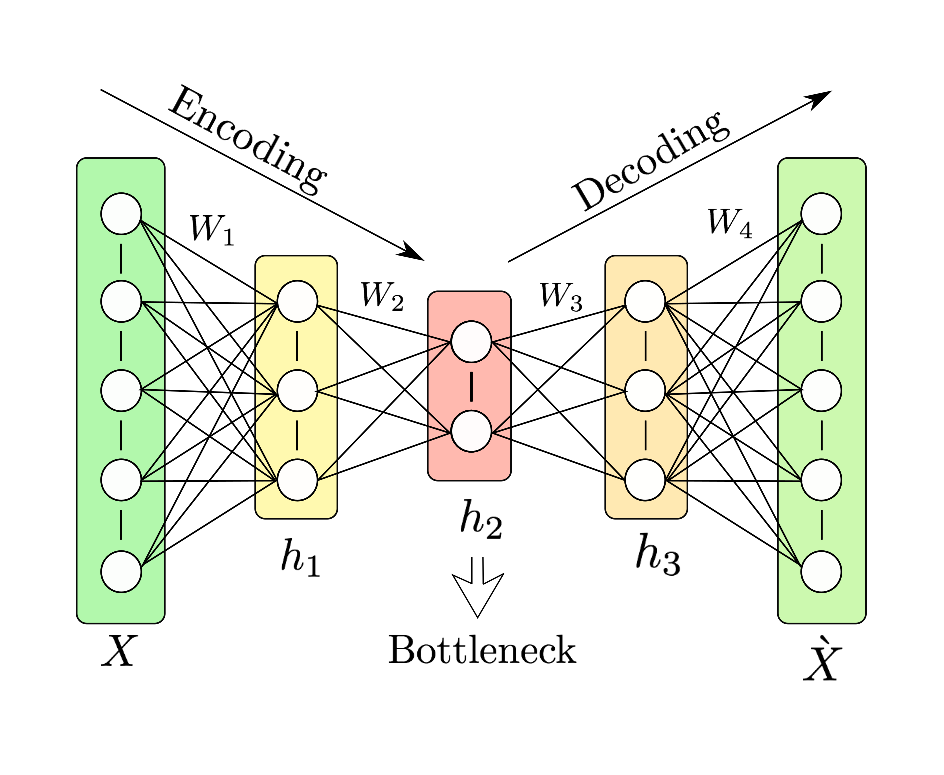
\includegraphics[width=240pt]{figure/fig_auto_encoder.eps}
  \caption{A small scale version of the Auto-Encoder. This network takes 5 dimensional input in the input layer. At each encoder layer, input is compressed into vector of lesser dimensions, lowest at the bottleneck layer.}
\label{autoEncoder}
\end{figure}


\section{Case Studies}\label{sec_example}
This sections presents two case studies presenting the effectiveness of our approach for path and motion synthesis applications.
\subsection{Path Generation}
In the design phase of a rehabilitation device that assists people stand from sitting position, it is required to generate linkages that can execute a sit-to-stand (STS) trajectory of hip as shown in Fig.~\ref{ex1_path}.
Table~\ref{hipPathTab} presents the discretized path data.
As our approach requires parametric representation of path, we first fit a cubic B-Spline with cord length parameterization through path data points to generate parametric curve shown in Fig.~\ref{ex1_path}.
We compute its path signature by the steps mentioned in Algorithm ~\ref{alg_signature} and raise the query for nearest neighbors among 1500 cluster centers of our database.
The distance metric for finding neighbors is $1-Cn_{max}$ in Eq.~\req{objectiveFunPath}.
Table~\ref{ex1_knnLinkageData} tabulates the link ratios corresponding to obtained nine nearest neighbors.
Next step is to compute actual parameters according to position, scale and orientation of the path.
It is done by comparing analogous points found by offset index $j$ in Eq.~\ref{nccEq}.
Figure ~\ref{ex1_solns} shows first eight fourbar mechanisms corresponding to nearest signatures to path signature of input.
As it can be clearly seen, these linkages generate highly accurate paths without any defects throughout sit to stand activity.

\begin{table}
\caption{Case Study 1 : Path Data}
\centering
\label{hipPathTab}
\begin{tabular}{cccccc}
\hline
Point & x & y & Point & x & y \\
\hline
1 & -7.81 & -9.65 & 10 & 0.28 & -1.31 \\
2 & -6.42 & -9.81 & 11 & 0.64 & 1.07 \\
3 & -5.14 & -9.62 & 12 & 0.98 & 2.73 \\
4 & -3.72 & -8.99 & 13 & 1.47 & 4.30 \\
5 & -2.62 & -8.14 & 14 & 2.73 & 6.58 \\
6 & -1.75 & -7.13 & 15 & 3.46 & 7.41 \\
7 & -0.91 & -5.67 & 16 & 4.07 & 7.95 \\
8 & -0.32 & -4.10 & 17 & 4.70 & 8.41 \\
9 & -0.02 & -2.92 & 18 & 5.32 & 8.76 \\
\end{tabular}
\end{table}

\begin{table}
\caption{Linkage Parameters of Nine Nearest Neighbor Paths}
\centering
\label{ex1_knnLinkageData}
\begin{tabular}{ccccccc}
\hline
  linkage & $l_1$ & $l_2$ & $l_3$ & $l_4$ & $l_5$ & $1 - Cn_{max}$ \\
\hline
 1 & 0.79 & 2.78 & 1.70 & 1.35 & -0.71 & 0.0011 \\
 2 & 1.59 & 1.28 & 0.96 & -1.74 & -1.13 & 0.0015\\
 3 & 0.99 & 0.71 & 1.66 & -1.07 & -0.85 & 0.0016\\
 4 & 0.51 & 0.48 & 1.11 & -0.02 & -0.15 & 0.0017\\
 5 & 0.93 & 0.75 & 2.18 & -1.65 & 0.96 & 0.0018 \\
 6 & 1.29 & 1.98 & 1.02 & -1.83 & -1.33 & 0.0019\\
 7 & 0.63 & 1.42 & 1.03 & -1.90 & -0.38 & 0.0020\\
 8 & 0.66 & 0.85 & 0.84 & -1.40 & -0.13 & 0.0021\\
 9 & 1.81 & 0.55 & 1.08 & 0.14 & -0.04 & 0.0022
\end{tabular}
\end{table}

\begin{figure}
\centering
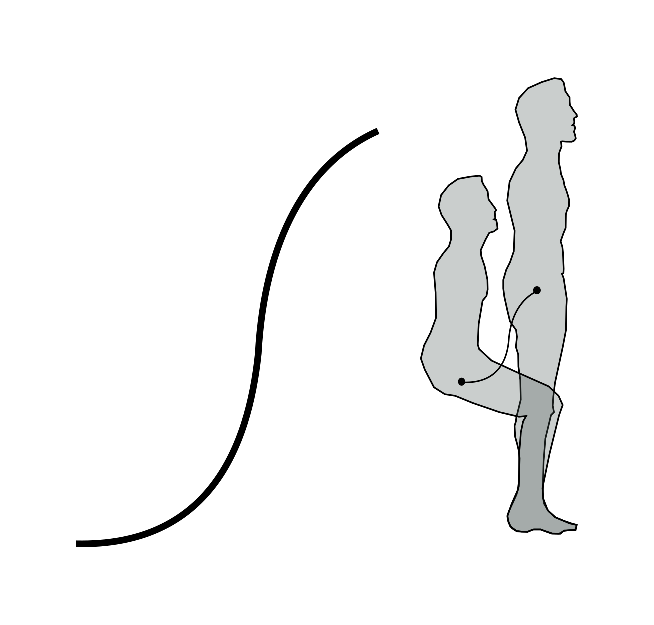
\includegraphics[width=240pt]{figure/path_solutions/hip_path.eps}
  \caption{Case Study 1: Path traced by hip joint during Sit-to-Stand Motion.}
\label{ex1_path}
\end{figure}

\begin{figure}
\begin{tabular}{cc}
  1)\putindeepbox[7pt]{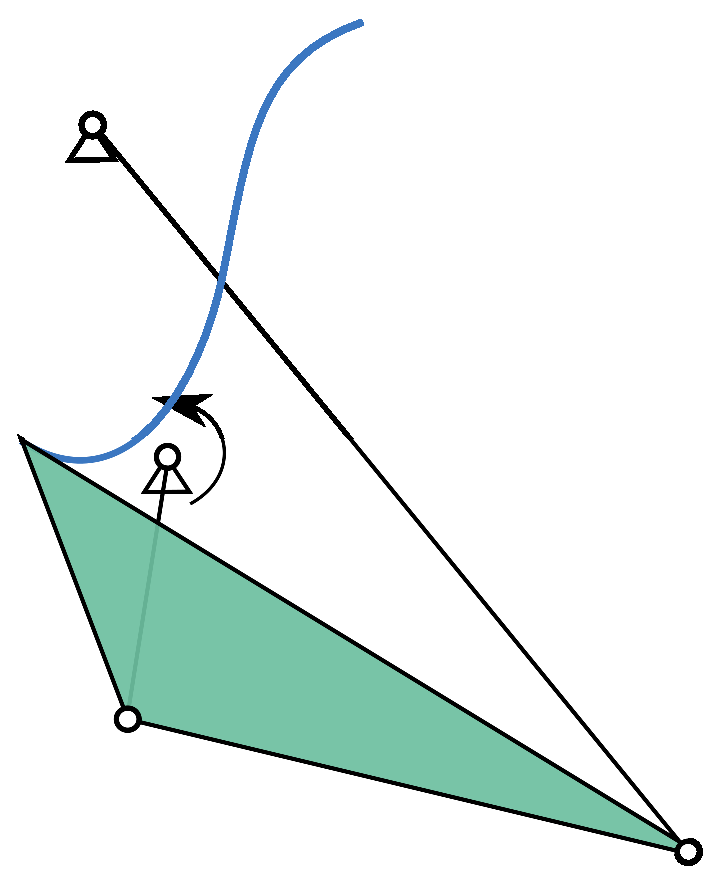
\includegraphics[width=100pt]{figure/path_solutions/path_sol1.eps}}
    & 2)\putindeepbox[7pt]{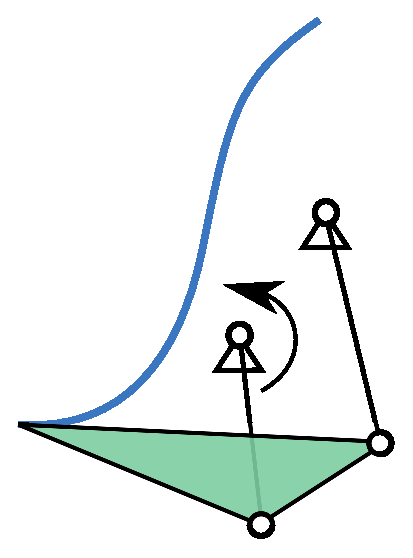
\includegraphics[width=60pt]{figure/path_solutions/path_sol2.eps}} \\
  3)\putindeepbox[7pt]{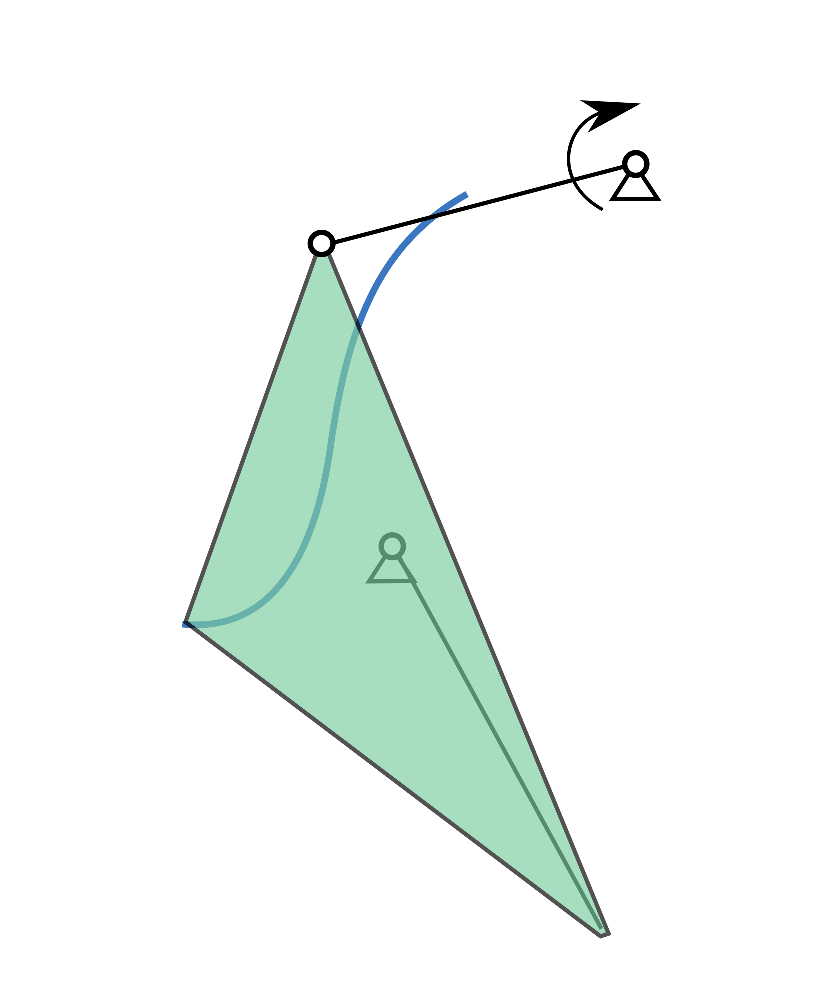
\includegraphics[width=120pt]{figure/path_solutions/path_sol3.eps}}
    & 4)\putindeepbox[7pt]{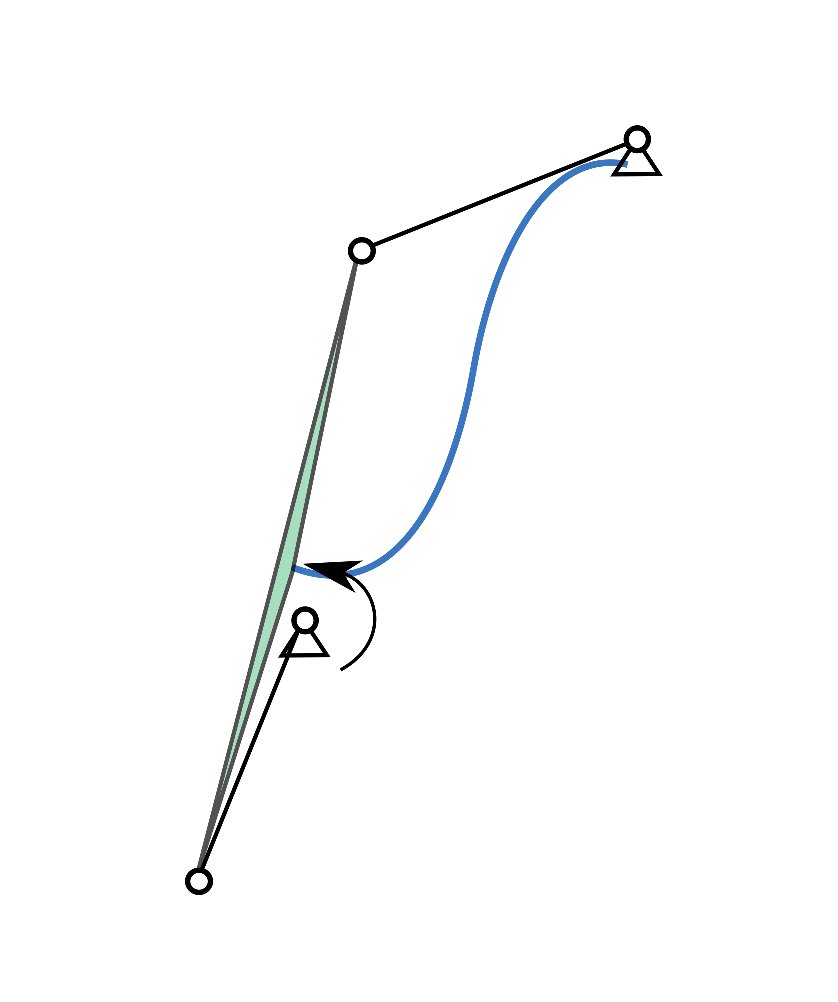
\includegraphics[width=120pt]{figure/path_solutions/path_sol4.eps}}\\
  5)\putindeepbox[7pt]{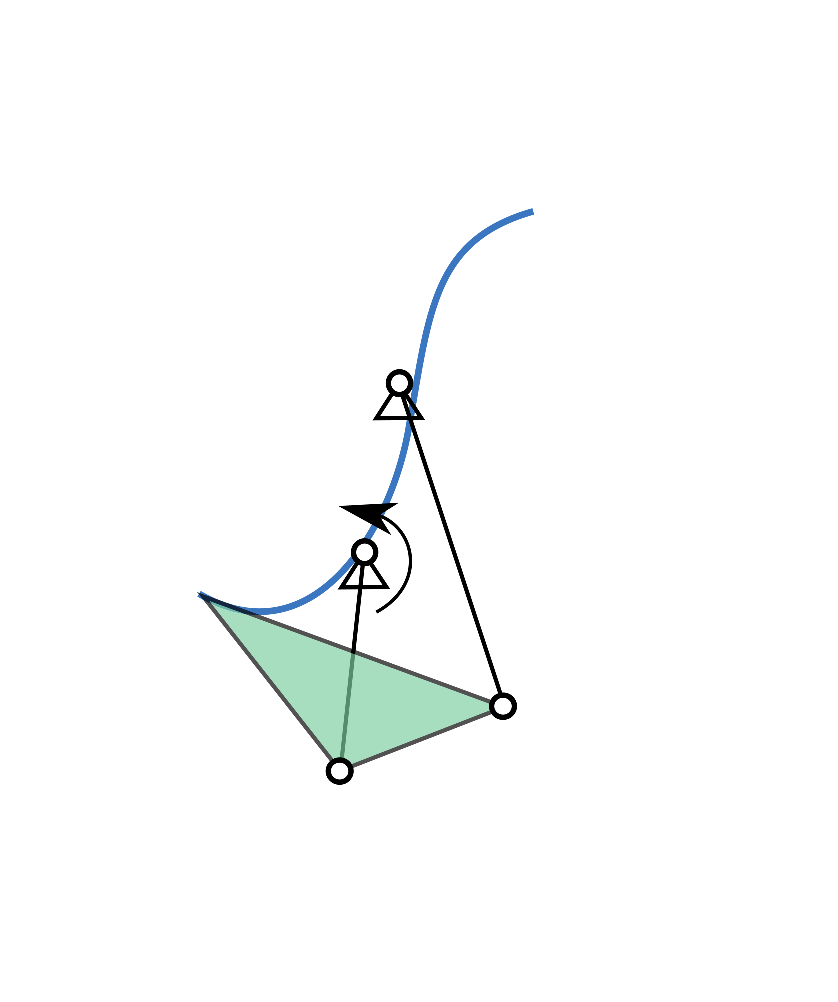
\includegraphics[width=120pt]{figure/path_solutions/path_sol5.eps}}
    & 6)\putindeepbox[7pt]{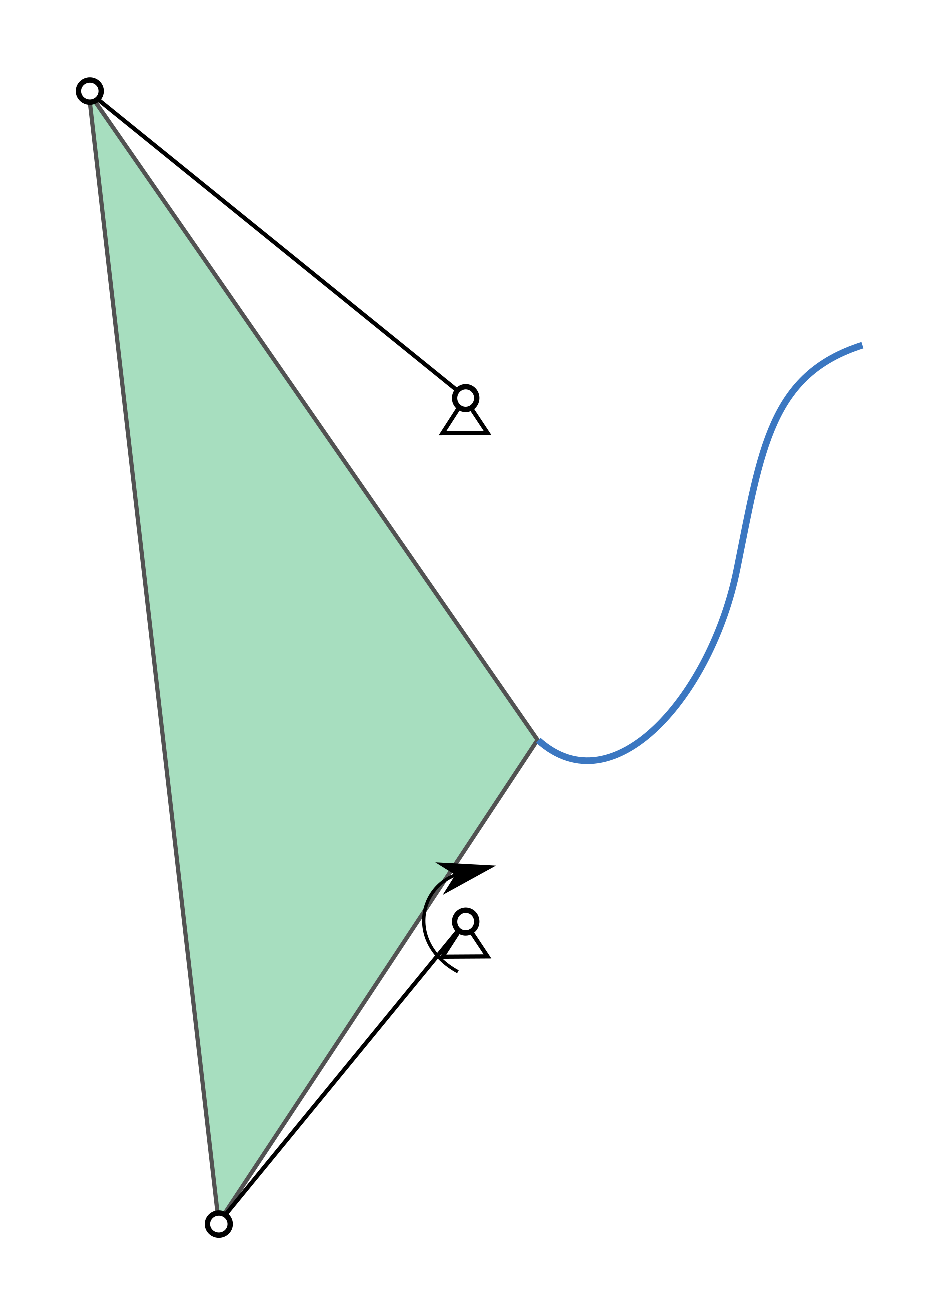
\includegraphics[width=120pt]{figure/path_solutions/path_sol6.eps}} \\
  7)\putindeepbox[7pt]{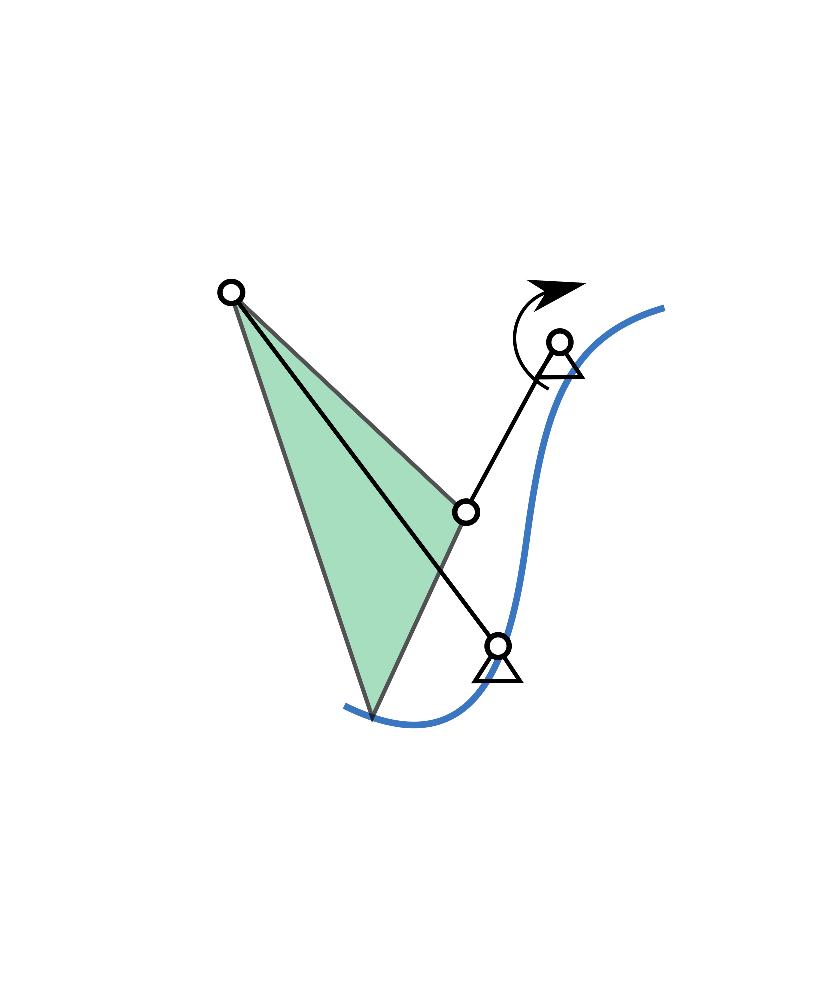
\includegraphics[width=120pt]{figure/path_solutions/path_sol7.eps}}
    & 8)\putindeepbox[7pt]{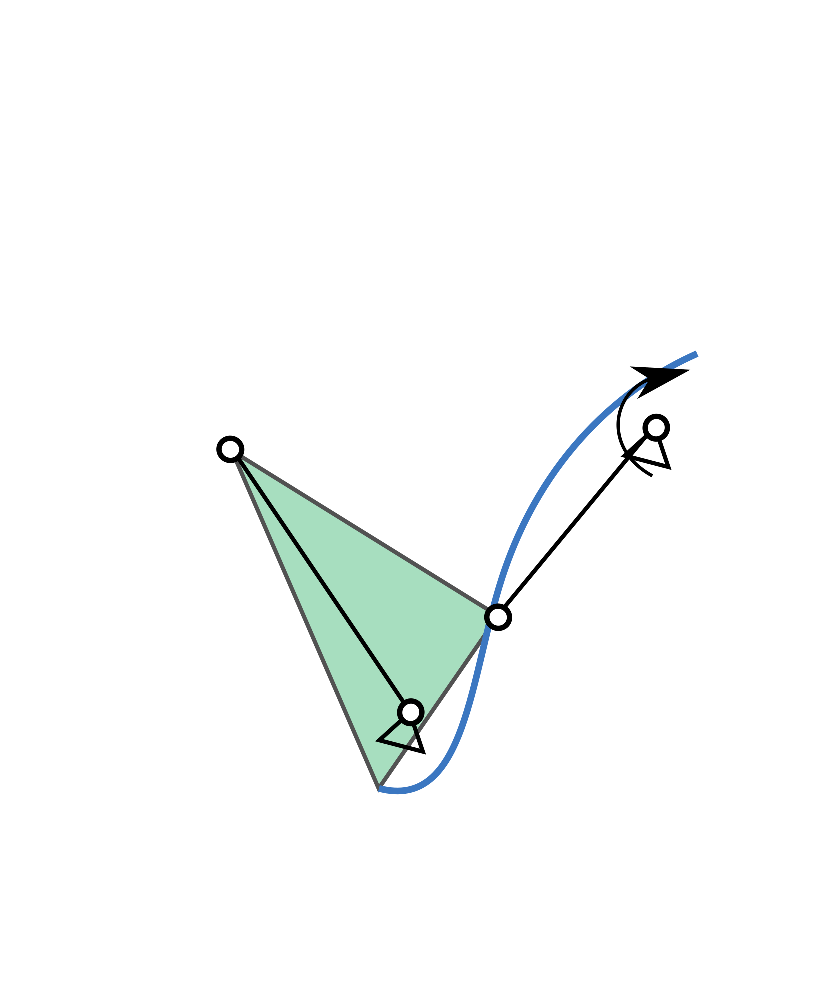
\includegraphics[width=120pt]{figure/path_solutions/path_sol8.eps}}\\
\end{tabular}
\caption{First 8 Linkages in the table~\ref{ex1_knnLinkageData} and their resultant coupler paths.}
\label{ex1_solns}
\end{figure}

\subsection{Motion Generation}
The task is to find a pool of linkage systems that can perform snow-shoveling with a motion shown in Fig.~\ref{motionQuery}.
The motion data is tabulated in Table ~\ref{poseData} to which we fit a B-spline with cord length parameterization in order to get parametric representation of motion.
The task can also be treated as a finite position motion generation and solved for valid solutions.
We try with our real time computational methods of algebraic fitting\cite{generalfitting-JCISE},\cite{deshpande2017} but obtained solutions suffer from circuit defect, which is not surprising as those methods do not account for continuity of the input positions.

Now we employ the approach presented in this paper.
First step is to calculate motion signature of the task motion using steps mentioned in Algorithm ~\ref{alg_signature}.
For that we follow the steps given in section~\ref{sec_sign} to obtain the motion signature depicted in Fig.~\ref{queryResult}.
Next we raise the signature query for nearest signatures among the cluster centers of the database.
Fig.\ref{queryResult} shows nine nearest neighbor signatures along with the task signature.
Table ~\ref{ex2_knnLinkageData} presents the linkage parameters corresponding to the nearest neighbors along with their distance score from the task.
Coupler motions of these linkages have a part, which matches with the shape of input motion query.
Actual scaling and orientation of the linkage can be found out easily by comparing analogous points, which are given by the offset index $j$ that corresponds to minimum distance$(E_min)$ in Eq.~\req{mccEq}.
Figure~\ref{ex2_solns} depict the solutions obtained after scaling and orienting the linkage to match required motion.
All of these linkages satisfactorily perform the input task without any defect.
As ground or fixed pivot locations should lie above the ground, all solutions except the $4^{th}$ solution are suitable for the task.
In light of these results, we can say that this approach produces a large variety of solutions, which otherwise would be very hard to find using precision point approach.

\begin{figure}
\centering
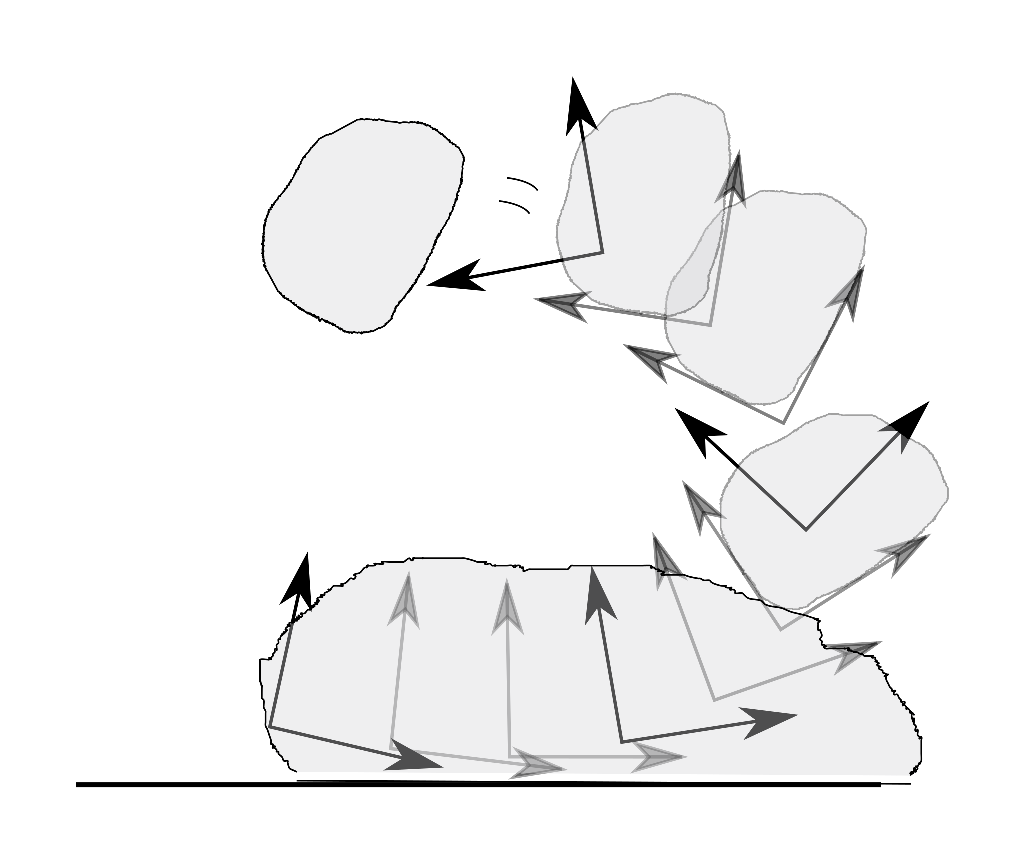
\includegraphics[width=240pt]{figure/fig_motion_query.eps}
  \caption{Case Study 2: User specified motion necessary for the snow shoveling task.}
\label{motionQuery}
\end{figure}

\begin{figure}
\centering
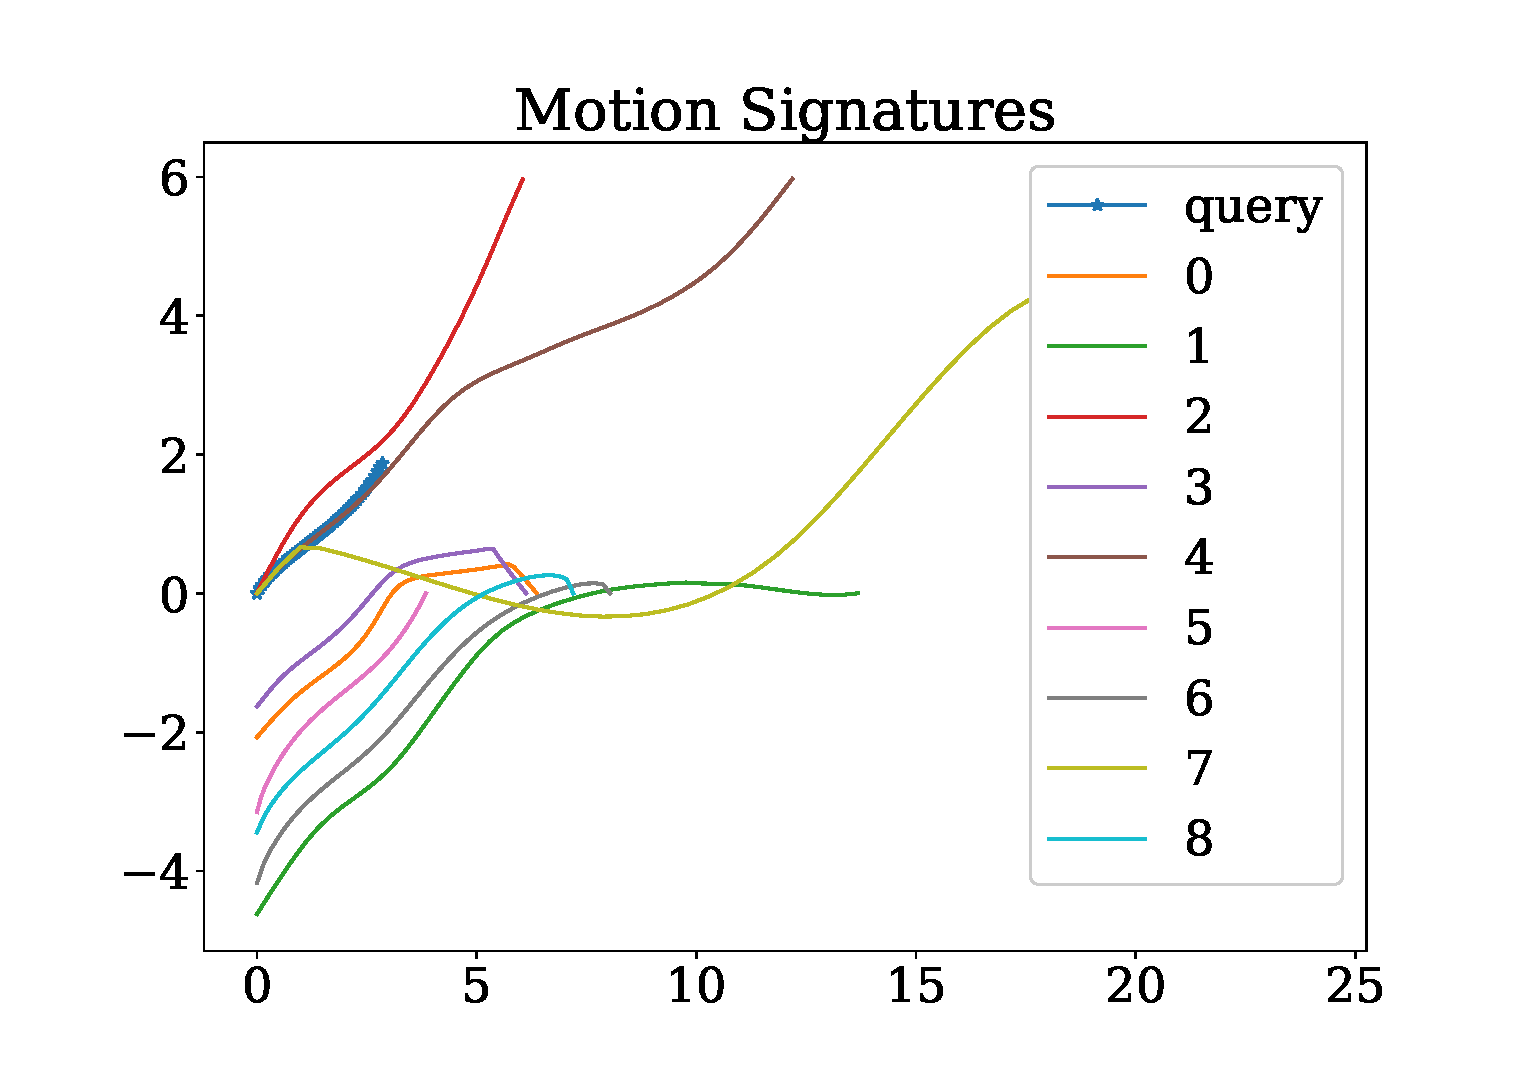
\includegraphics[width=240pt]{figure/fig_ex_motion_signatures.eps}
  \caption{Case Study 2 - Query Result: Motion signatures in the dataset with highest similarity.}
\label{queryResult}
\end{figure}


\begin{table}
\caption{Case Study 2: Pose Data}
\centering
\label{poseData}
\begin{tabular}{cccccccc}
\hline
%Pose & x & y & $\theta$ \\
Pose & x & y & $\theta$ & Pose & x & y & $\theta$ \\
\hline
1 & 0.03 & 0.07 & 6.06 & 6 & 1.39 & 0.47 & 0.73 \\
2 & 0.38 & 0.01 & 6.18 & 7 & 1.36 & 0.77 & 1.03 \\
3 & 0.71 &-0.00 & 0.04 & 8 & 1.18 & 1.06 & 1.36 \\
4 & 1.02 & 0.06 & 0.22 & 9 & 0.88 & 1.27 & 1.74 \\
5 & 1.26 & 0.22 & 0.46 & \\
\end{tabular}
\end{table}

\begin{table}
\caption{Case Study 2: Linkage Parameters corresponding to Nine Nearest Neighbor Motions}
\centering
\label{ex2_knnLinkageData}
\begin{tabular}{ccccccc}
\hline
  linkage & $l_1$ & $l_2$ & $l_3$ & $l_4$ & $l_5$ & $E_{min}$ \\
\hline
 1 & 1.28 & 0.88 & 1.77 & -1.32 & 1.79 & 0.0186   \\
 2 & 1.05 & 1.14 & 1.09 & 0.35 & -0.60 & 0.0362   \\
 3 & 2.06 & 2.28 & 1.84 & -1.71 & 0.51 & 0.0378   \\
 4 & 1.52 & 1.22 & 1.46 & 0.05 & 0.12 & 0.0402    \\
 5 & 1.12 & 0.99 & 0.57 & 0.05 & 0.68 & 0.0467    \\
 6 & 1.58 & 0.88 & 1.17 & 0.08 & -0.22 & 0.0481   \\
 7 & 2.17 & 0.38 & 2.87 & -3.51 & 1.39 & 0.0578   \\
 8 & 1.55 & 0.79 & 0.85 & -0.80 & -0.52 & 0.0585  \\
 9 & 0.91 & 1.40 & 1.93 & -0.93 & -0.83 & 0.0605
\end{tabular}
\end{table}

\begin{figure}
\begin{tabular}{cc}
  1)\putindeepbox[2pt]{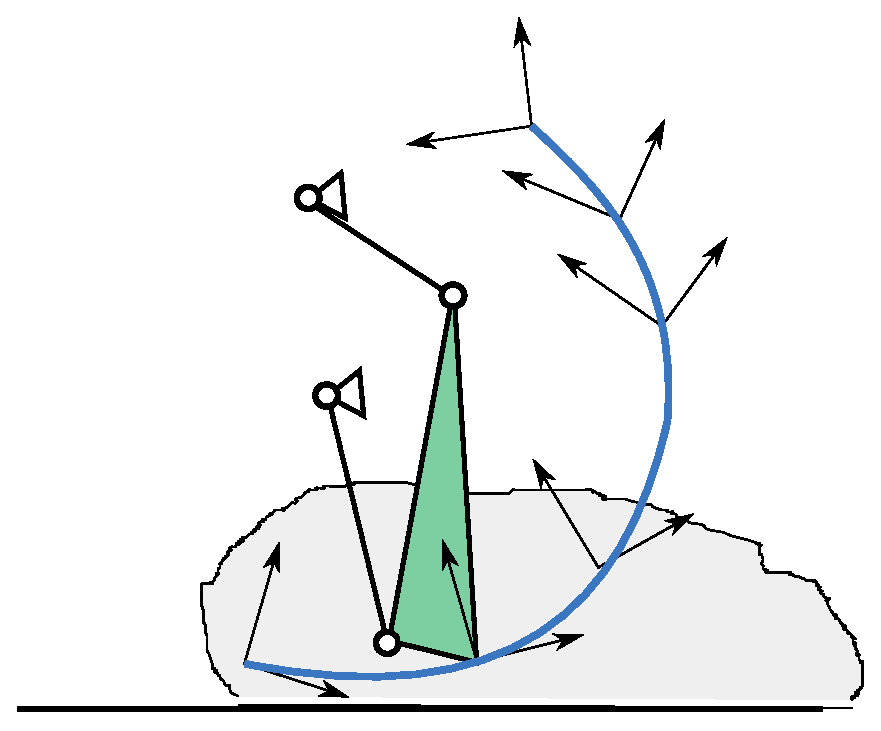
\includegraphics[width=120pt]{figure/sol1.eps}}
    & 2)\putindeepbox[2pt]{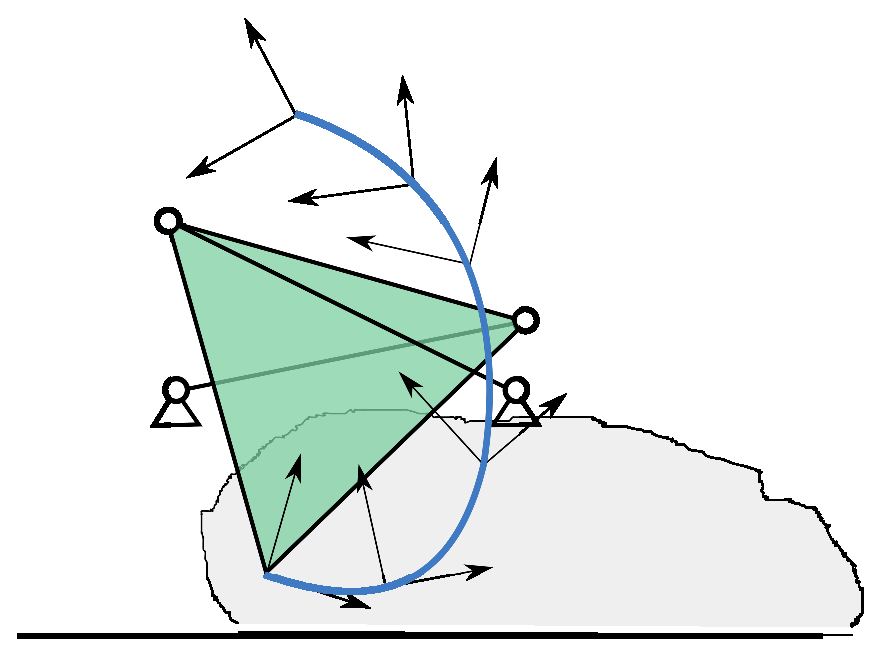
\includegraphics[width=120pt]{figure/sol2.eps}} \\
  3)\putindeepbox[2pt]{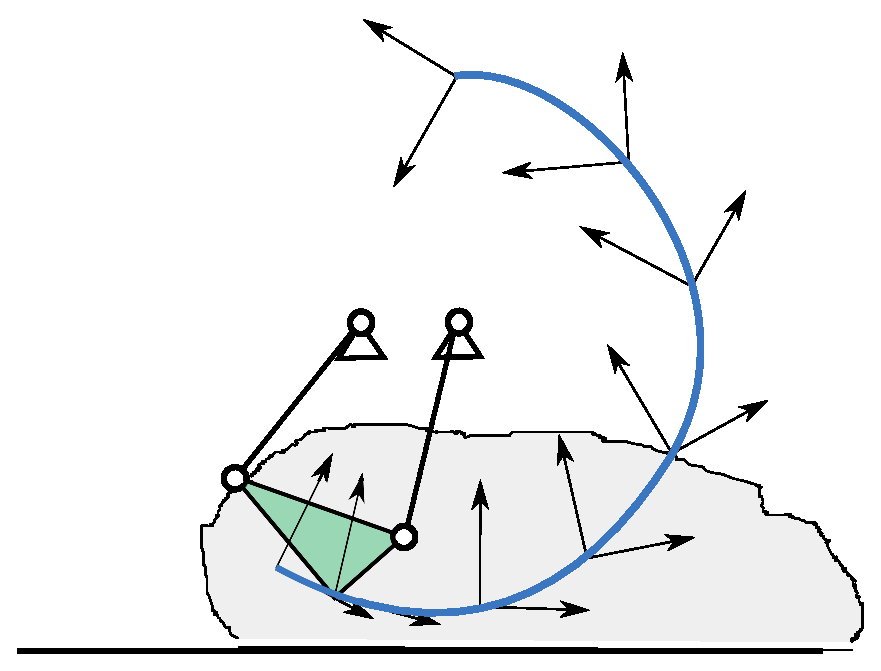
\includegraphics[width=120pt]{figure/sol3.eps}}
    & 4)\putindeepbox[2pt]{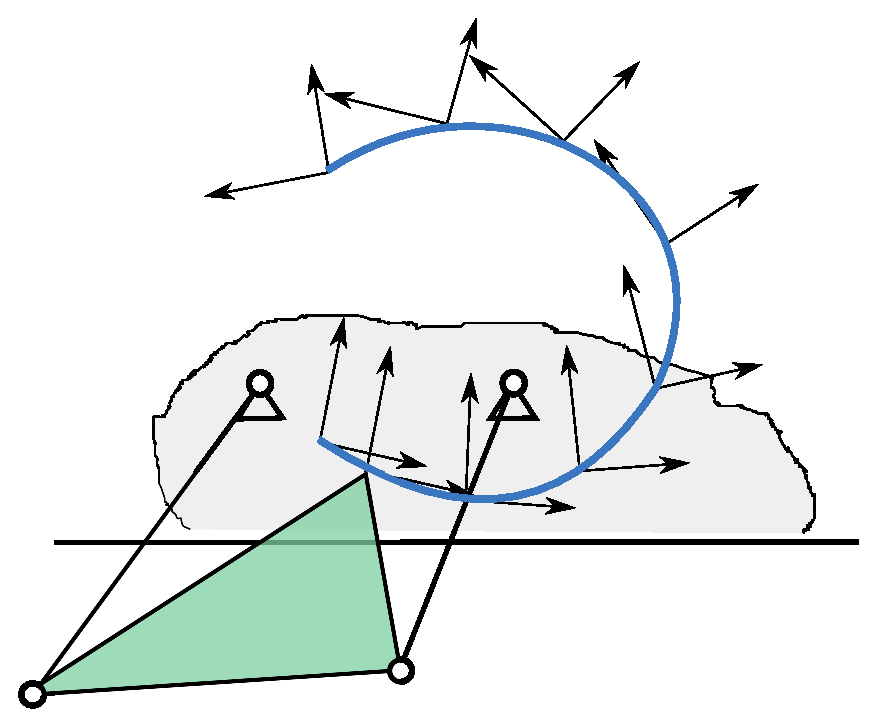
\includegraphics[width=120pt]{figure/sol4.eps}}\\
  5)\putindeepbox[2pt]{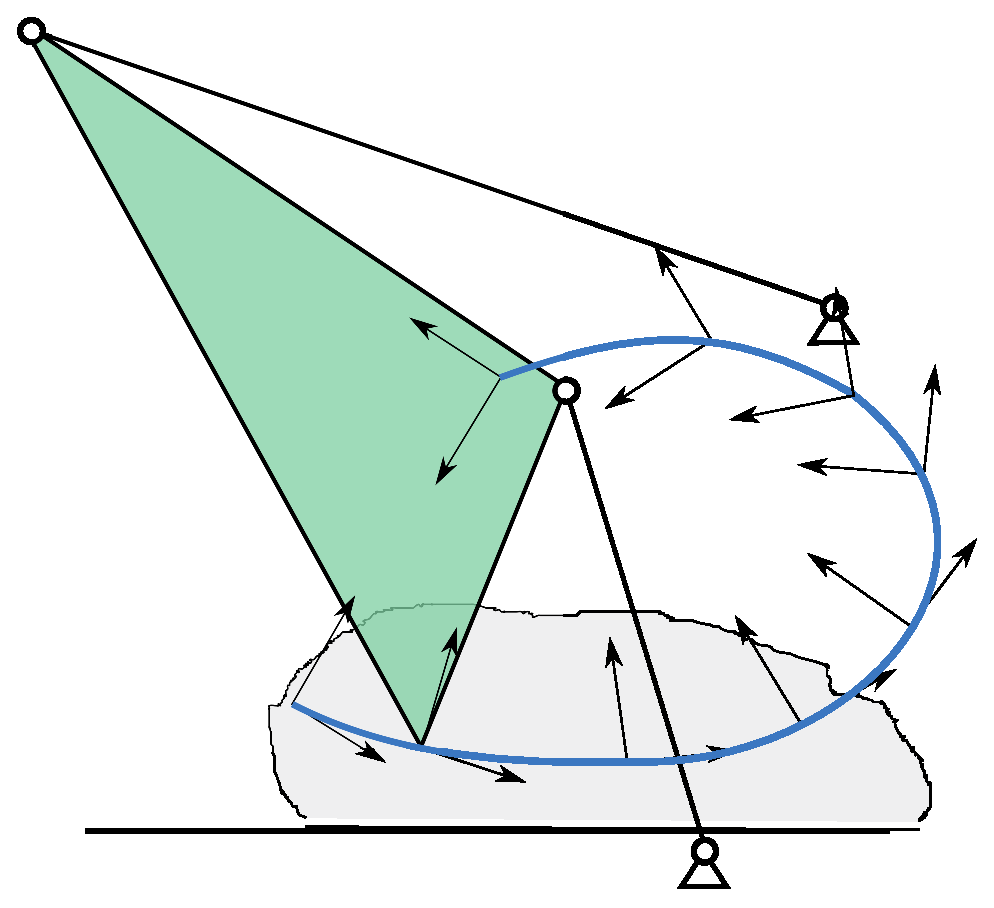
\includegraphics[width=120pt]{figure/sol6.eps}}
    & 6)\putindeepbox[2pt]{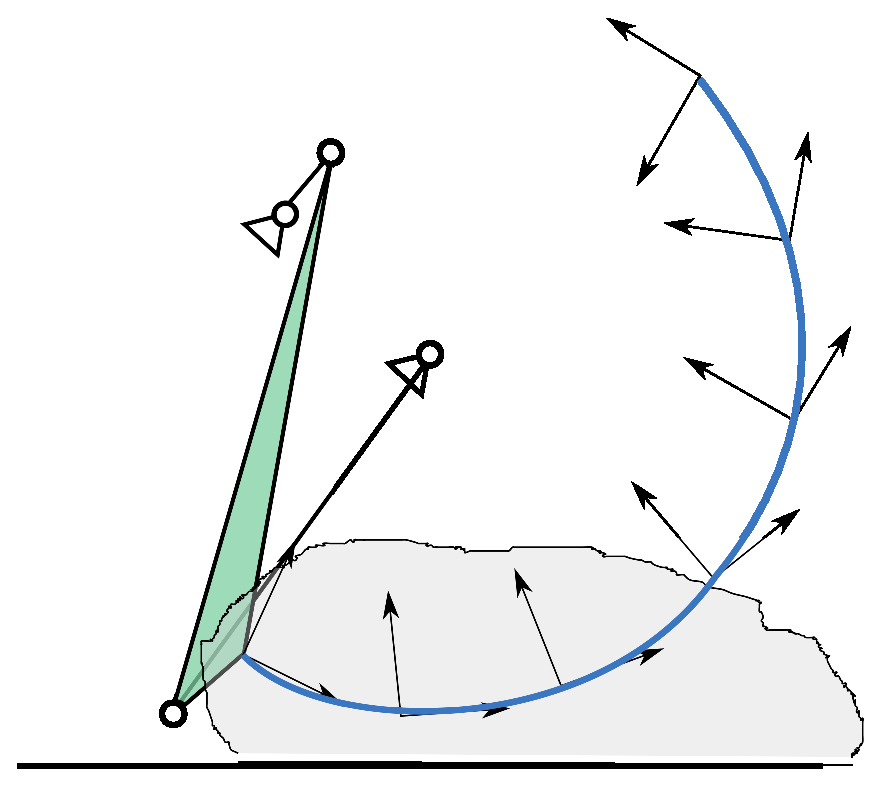
\includegraphics[width=120pt]{figure/sol7.eps}} \\
  7)\putindeepbox[2pt]{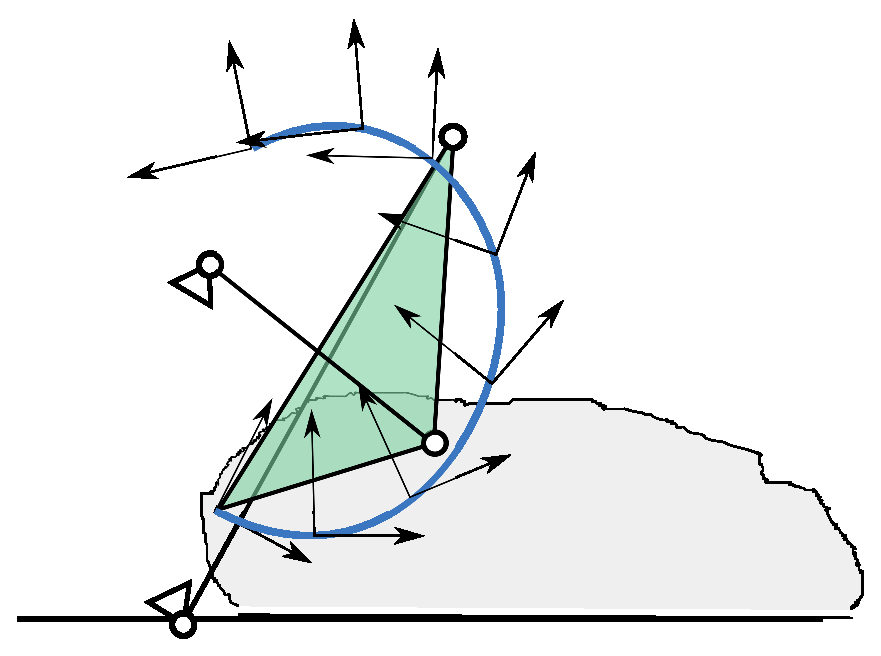
\includegraphics[width=120pt]{figure/sol8.eps}}
    & 8)\putindeepbox[2pt]{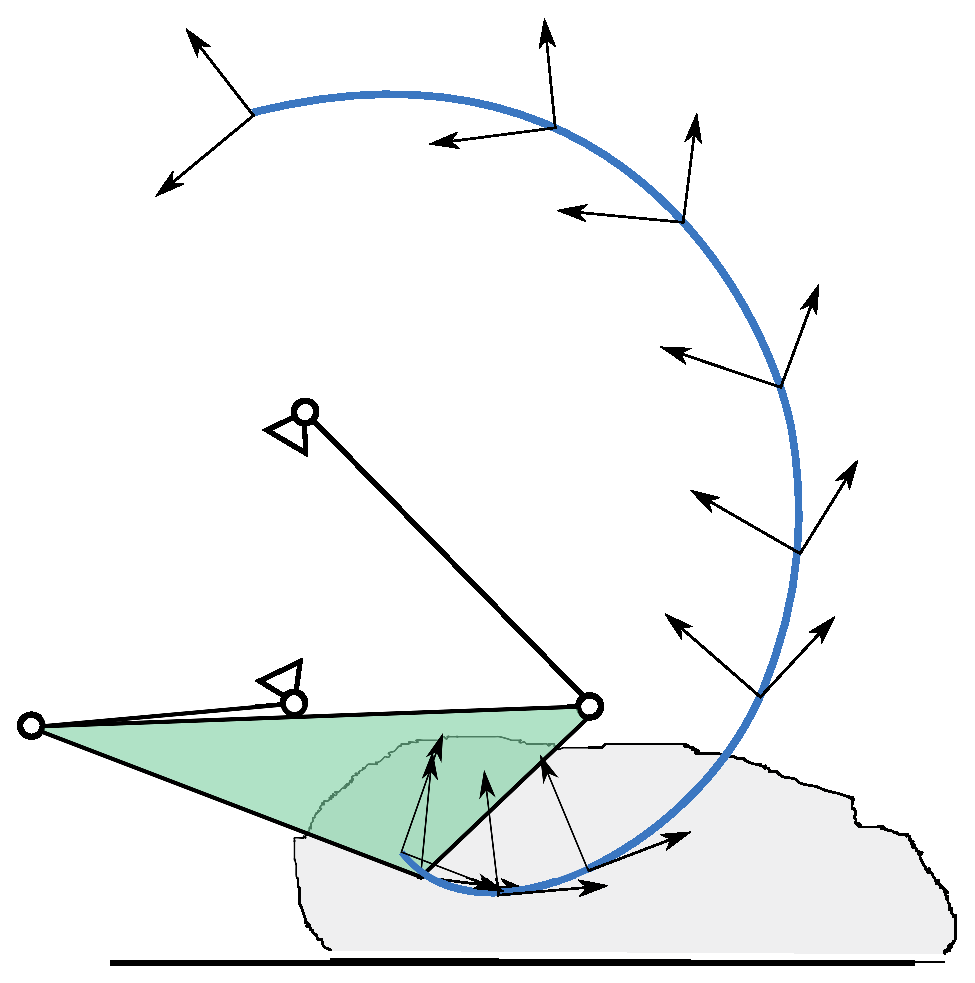
\includegraphics[width=120pt]{figure/sol9.eps}}\\
\end{tabular}
\caption{Case Study 2: First 8 Linkages in the table~\ref{ex2_knnLinkageData} and their resultant coupler motions.}
\label{ex2_solns}
\end{figure}


\section*{Conclusion}
This approach presents a novel optimization approach towards defect free linkage synthesis.
The framework is highly data efficient due to similarity invariant representation of paths and motion, which also facilitates partial matching.
The method always returns defect free solutions as it is inherently taken care of.
Sensitivity analysis indicates that complexity of the objective function, although obviously multimodal and nonlinear, is not overly complex and certainly well behaved in the singular spaces.
Hierarchically clustered database provides efficient query search.
Finally, the effectiveness of presented approach is showcased by two case studies for each of which nine defect free solutions were found.
Although our method can provide highly accurate results, our focus here is to generate high number of defect free solutions that can perform the task in more or less similar fashion;
because more often than not, linkage synthesis algorithms are desired to be prolific in terms of concept generation than to produce highly accurate very few solutions.

\begin{acknowledgment}
This work has been financially supported by National Science Foundation under a research grant to Stony Brook University (A. Purwar and Q.J. Ge, grant CMMI-1563413). All findings and results presented in this paper are those of the authors and do not represent those of the funding agencies.
\end{acknowledgment}

\bibliographystyle{purwar}
\bibliography{References}
\newpage
\clearpage
\listoftables
\listoffigures

\end{document}
